\chapter{Simulation and Event Reconstruction for the ATLAS Experiment}

In current LHC pp collison, bunches of protons collide every 25 nanoseconds (ns), which gives a large challenge to event reconstruction and selections.
To predict and model each process, the Monte Carlo simulations of physics events are essential for high-energy physics experiments.
This section will briefly discuss the event simulation and reconstruction programs based on the ATLAS software framework. 

\section{Event sumilation}
%\subsection{Simulation framework}

The ATLAS simulation program is integrated into the ATLAS software framework called \textit{Athena}~\cite{atlas:athena},
which uses Python as an object-oriented scripting and interpreter language to configure and load C++ algorithms and objects.
Figure~\ref{fig:frame_overview} shows the overview of ATLAS simulation data flow~\cite{Aad:2010ah}.
In the diagrams, the square-cornered boxes represents algorithms and applications to be run and round-cornered boxes denote data objects.
\begin{figure}[!htb]
  \centering
  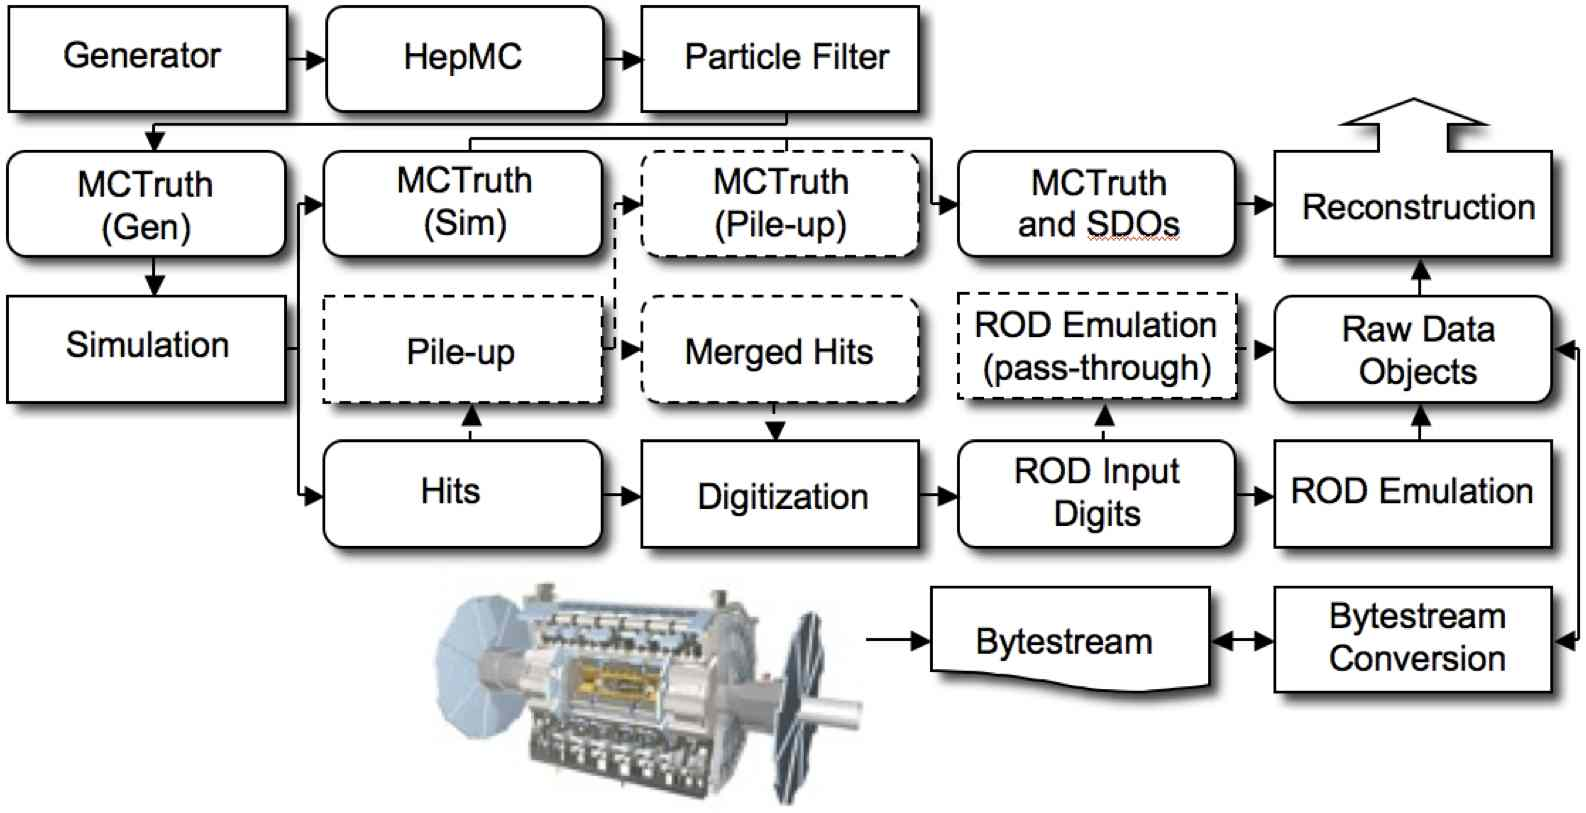
\includegraphics[width=1.0\textwidth]{figures/Simulation/outline_atalsSimulation_v2.png}
  \caption{The flow of the ATLAS simulation software.}
  \label{fig:frame_overview}
\end{figure}

First of all, events are produced by MC generators in standard HepMC format and then read into the simulation.
During the simulation, particles are propagated through the full ATLAS detector whose configurations can be set by users via GEANT4 toolkit.
The energies deposited in the sensitive regions of the detector are recorded as \textit{hits} that contains the total energy deposition,
position and time, and are written to a simulation hit file.
In the meatime, the events in "truth" format are also recorded to contain the history of the interactions from the generator, including incoming and outgoing particles.
Simulated Data Objects (SDOs) are created from truth, which are maps between hits in sensitive portions of the detector and truth information of particles in simulation.
The files are then sent to digitization, with constructs ``digits" inputs and be written into Raw Data Object (RDO) file used for reconstruction.

In conclusion, there are three main parts of framework: \textit{Generation}, \textit{Simulation} and \textit{Digitization}.
More details are given as below:

\textbf{Event generation}

As shown in figure~\ref{fig:mc_event_structure}~\cite{Hoche:2014rga}, at hardon colliders, multiple scattering and rescattering effects arise, which needs to be simulated by Monte Carlo (MC) event generators to reflect the full complexity of those event structures.
Several MC event generators can be used to generate events originally in HepMC format.
The events can be filtered at generation time with some certain requirements (eg. decay channel or missing energy above a certain threshold).
The generator is responsible for any prompt decays (e.g. W or Z bosons) but stores any "stable" particle expected to propagate through a part of the detector. 
During the generation steps, any interactions with detector are ignored and only immediate decays are considered.

There are several MC generators that have been widely used with general purpose, which include \textsc{Sherpa}~\cite{Gleisberg_2009}, \textsc{Herwig++}~\cite{Bahr2008}, \textsc{PowhegBox}~\cite{Nason:2004rx}, \textsc{MC@NLO}~\cite{Frixione_2002} and \textsc{Pythia8}~\cite{Sjostrand:2007gs}.

\begin{figure}[!htb]
  \centering
  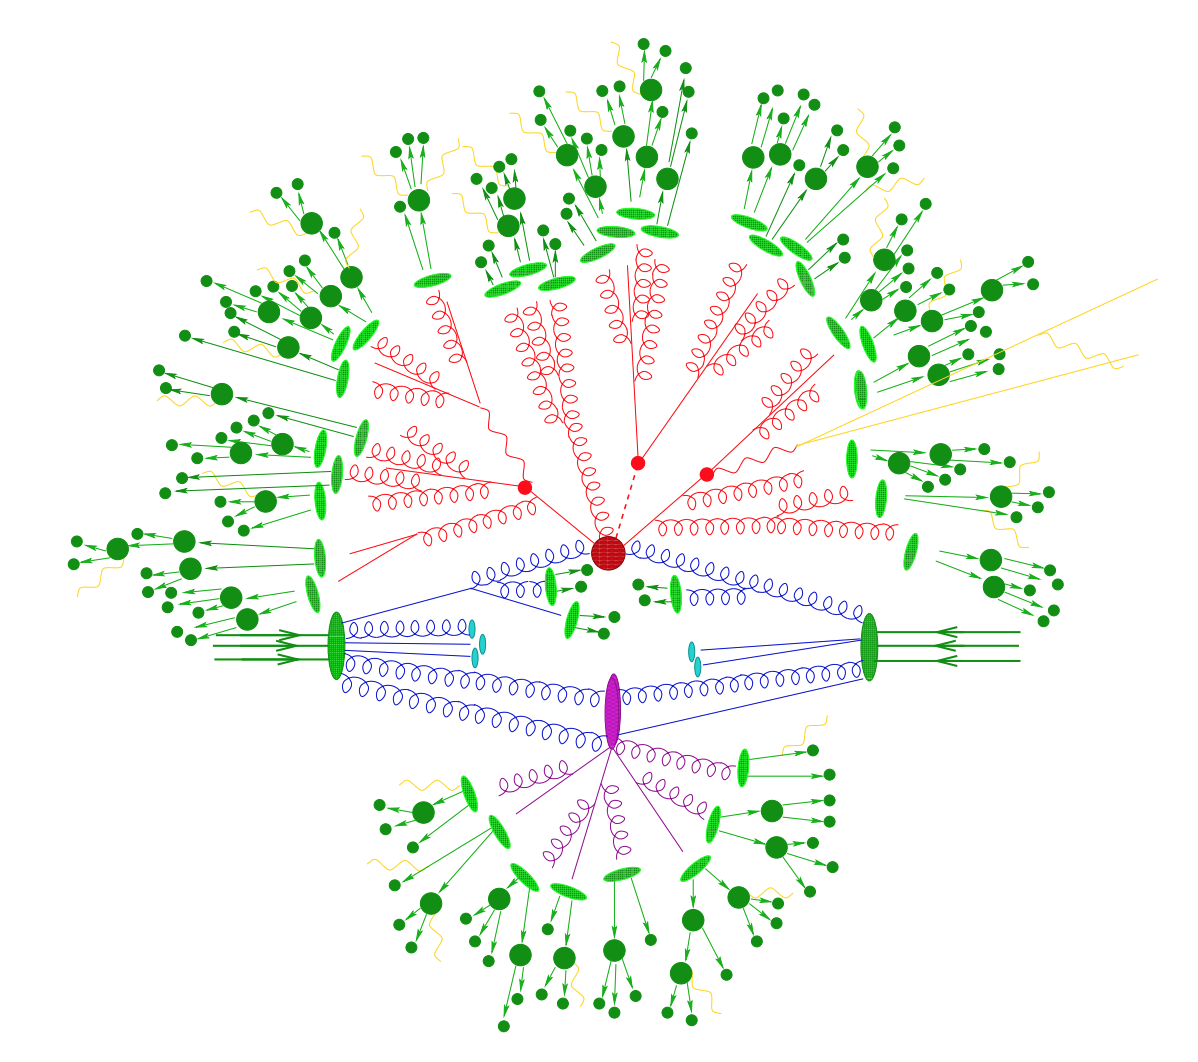
\includegraphics[width=0.7\textwidth]{figures/Simulation/mc_event_structure.png}
  \caption{Sketch of a hardon-hardon collision simulated by MC event generator. The red blob in center denotes the hard collision, surrounded by tree-like structures representing Bremsstrahlung which is simulated by Parton Showers. The purple blob stands for a secondary hard scattering event. The light green blobs indecate the parton-to-hardon transitions and the dark green blobs represents hardon decays. The yellow lines are soft photon radiations.}
  \label{fig:mc_event_structure}
\end{figure}

\textbf{Simulation}

GEANT4 is used as standard simulation toolkit for the ATLAS experiment, which transports physics particles through the detector's geometry.
During the generation level, the entire connected chain of the HepMC event is stored as the Monte Carlo truth. 
Only the stable particles are read into GEANT4 for further simulation and selection, while transformations can be applied to these events to select certain processes.
During the simulation, many secondary tracks can be produced, therefore only information from the interactions of interest are stored, including the incoming particles, step sequence, vertex as well as outgoing particles.
The output of GEANT4 is called \textit{hit file}, which contains metadata describing the configuration of the simulation during the run, all truth information requested and a collection of hits for each subdetector.

Since the standard ATLAS detector simulation cost very large computing resources to accurately model the complex detector geometry and physics descriptions, some fast simulation programss are developed according to different user purpose.
Some popular fast-sim toolkits include \textit{Fast G4 Simulation}~\cite{Barberio:2007gba}, \textit{ATLFAST-I}~\cite{Richter-Was:683751} and \textit{ATLFAST-II}~\cite{Edmonds:1091969}.

\textbf{Digitization}

The hit outputs from simulated events, including hard scattering signal, minimum bias, beam halo, beam gas and cavern background events, are then sent into digitization procedure, converted into detector response called ``digits".
Before converted into detector signal as `digits' formart, each type of event can be overlaid at a user-specified rate.
Those overlay, called ``pile-up", can be done during degitization to save the CPU time.
At this stage, the detector noise and the first level trigger that implemented with hardware on the real detector are added into events.
The digitization firstly constructs ``digits" inputs to the readout drivers (RODs) in the detector electronics.
Then the ROD functionality is emulated, and the output digits are written out as Raw Data Object (RDO) file.
In addition, the digitization algorithms can also produce Simulated Data Objects (SDOs), which contain information about all the particles, noise and the amount of energy that contributed to the signal. 
Then all information are sent into reconstruction level described in next subsection.

%\subsection{Simulation framework}

\section{Event reconstruction}

The data flow of ATLAS data processing is sketched in figure~\ref{fig:data_processing}\cite{Boyd_2010}. 
Data from detector is firstly filtered by online trigger system and then send to the \textit{Tier-0 (T0)} for initial processing by offline reconstruction software also based on Athena.
A small amount of data named "express stream" is processed in almost real time in T0 for online data quality monitoring.
In addition, some other dedicated data steams are sent out at trigger level for detector alignment and calibration.
These calibration and alignment information are then used for bulk reconstruction in T0.
At the end of the reconstruction chain, the data are delivered into \textit{Tier-1 (T1)} and \textit{Tier-2 (T2)} centers for further analysis and production of simulated data.
Besides, T1 centers are also responsible for data reprocessing by re-running data reconstruction with improved calibration and alignment constants and with improved reconstruction algorithms.
This section describes the reconstruction of some important physics objects in ATLAS experiment, i.e. tracks, vertices, electrons, muons, jets, and missing energies.
\begin{figure}[!htb]
  \centering
  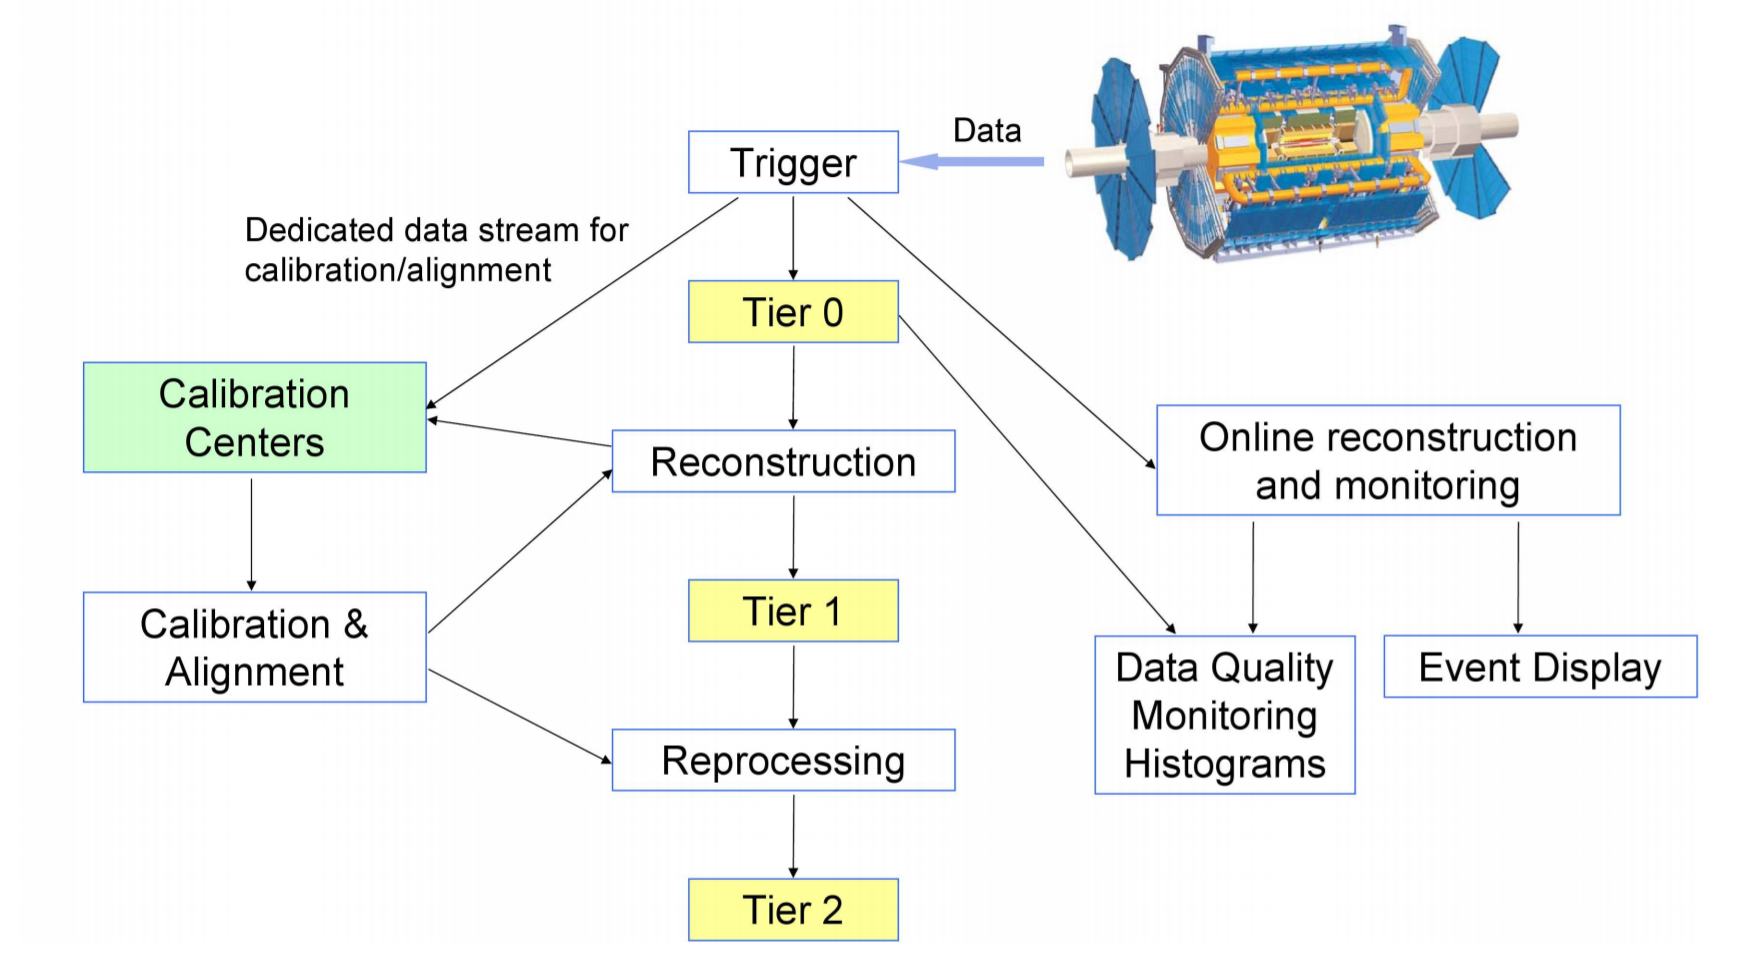
\includegraphics[width=0.9\textwidth]{figures/Simulation/data_processing.png}
  \caption{The flowchart of the ATLAS data processing.}
  \label{fig:data_processing}
\end{figure}

\subsection{Track}
\label{sec:track}

The ATLAS detector is composed of two independent tracking systems: the Inner Detector (ID) close to the interaction point, and the Muon Spectrometer (MS) located in the outermost region.
The reconstructed charged-particle trajectories in the ID and MS are referred to as ID tracks and MS tracks respectively.
The challenge of ID reconstruction is that it needs to handle high track density that imposes a large number of combinatorial track candidates, 
while the MS reconstruction is however largely limited by the huge amount of inert material, the large background and the highly inhomogeneous magnetic field~\cite{Cornelissen:1020106}.
More details of these two types of track are given as below:

\textbf{Inner detector track}

Figure~\ref{fig:track_ID} sketches the ID system used for detecting charge-particle tracks.
The ID track reconstructions contains two sequences: \textit{inside-out} track reconstruction and \textit{outside-in} one.
\begin{figure}[!htb]
  \centering
  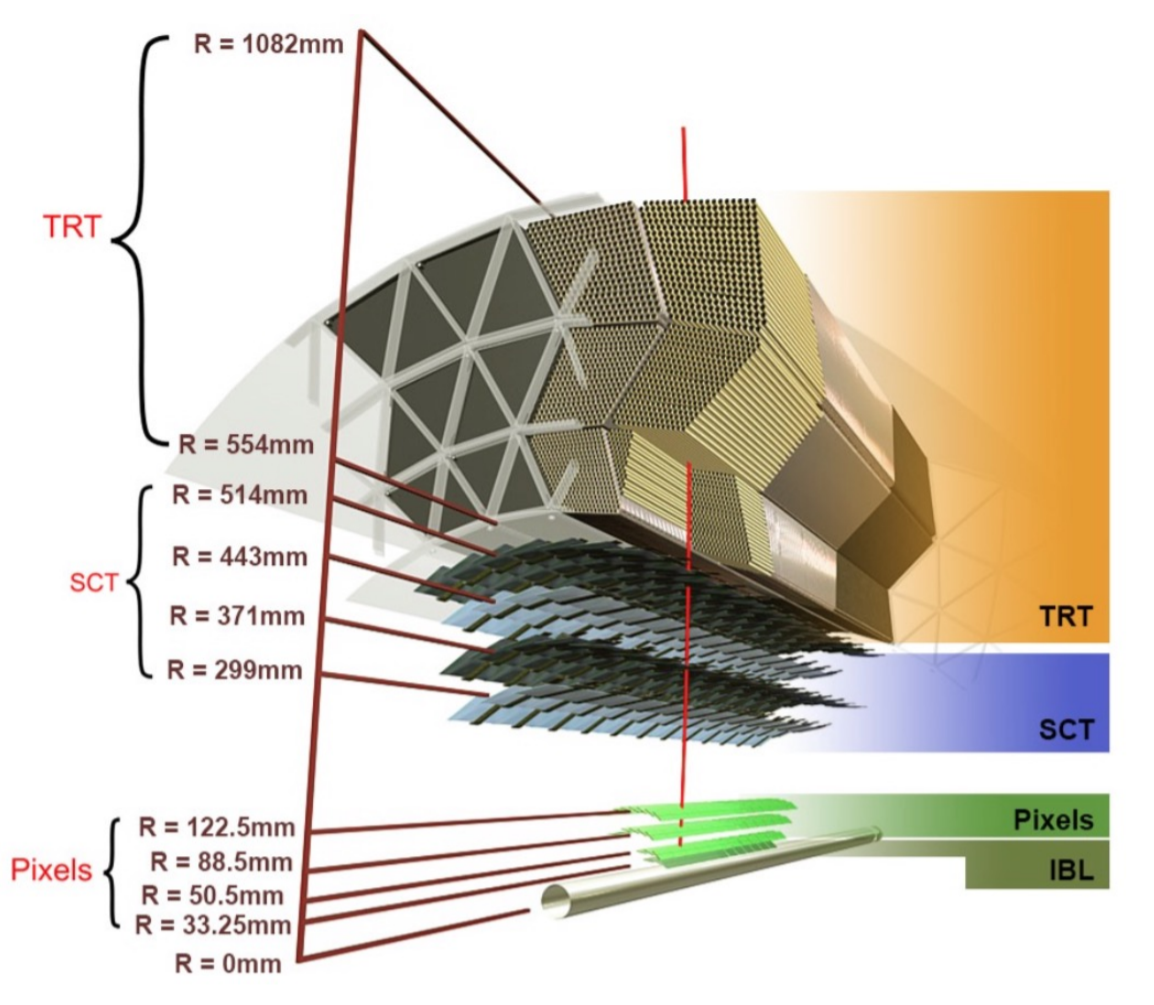
\includegraphics[width=0.7\textwidth]{figures/Simulation/track_ID.png}
  \caption{Schematic view of the ATLAS inner detector showing all the corresponding components.}
  \label{fig:track_ID}
\end{figure}

For inside-out tracking, it exploits the high granularity of the pixel and SCT detectors to discover prompt tracks originating from the interaction point.
In first step, the track seeds are formed by combining the information of space-points in the three pixel layers and the first SCT layer.
Then, these seeds are extended throughout the SCT to build track candidates.
After that, these candidates are fitted with some quality cuts applied to remove the outlier clusters, reject the fake tracks and resolve ambiguities in the cluster-to-track association.
The selected tracks are then further extended to TRT, and refitted with the full information from pixel, SCT and TRT detectors.

Another complementary approach, outside-in, searches for unused track segments start from TRT instead.
These segments are then extended into the SCT and pixel detectors to improve the tracking efficiency for secondary tracks from conversions or decays of long-lived particles.

\textbf{Muon spectrometer track}

The MS track reconstruction\cite{Aad:2016jkr} starts from searching hit patterns inside each muon chamber to form segments.
In each MDT chamber and nearby trigger chamber, a Hough transform\cite{ILLINGWORTH198887} is used to search the hits lie on a certain trajectory in the bending plane of the detector.
The MDT segments are reconstructed by performing a linear fit to the hits found in each layer.
The RPC or TGC hits can be built by measuring the coordinate orthogonal to the bending plane.
And the segments of CSC can be built using a separate combinatorial search in the $\eta$ and $\phi$ detector planes.

Then muon track candidates are built by fitting hits from segments in different layers together.
This task makes use of the algorithm by performing a segment-seeded combinatorial search, which starts by using the segments generated in the middle layers of the detector where more trigger hits are available as seeds.
The search is then extended to use the segments as seeds from the inner and outer layers.
The segments are selected based on criteria of hit multiplicity and fit quality, and are matched using their relative positions and angles.
To build a track, at least two matching segments are required, except in the barrel-endcap transition region where a single high-quality segment with $\eta$ and $\phi$ information can be used to build a track.
At beginning, the same segment can be used to build more than one track candidates.
Later on, an overlap removal algorithm is performed to select the best assignment to a single track, or decide whether allows the certain segment to be shared between two tracks.

The hits associated with each track candidate are then fitted using a global $\chi^{2}$ fit.
The algorithm accepts the track candidate if its fitting $\chi^{2}$ passes the selection criteria.
Hits contribute largely to $\chi^{2}$ are removed and the track fit is repeated.
In addition, the algorithm performs a hit recovery procedure that looks for additional hits consistent with the candidate trajectory, and the track candidate is refit if additional hits are found.

\subsection{Primary vertex}

The primary vertex (PV) is reconstructed by using the reconstructed tracks introduced in previous section as inputs.
The tracks to be considered for vertex reconstruction must satisfy the following criterias\cite{ATL-PHYS-PUB-2015-026}:
\begin{itemize}
	\item $p_{T} > 400$ MeV
	\item $|\eta| < 2.5$
	\item Number of silicon hits 
$\geq 
\begin{cases}
9&  \text{if} |\eta|\leq1.65\\
11& \text{if} |\eta|>1.65
\end{cases}$
	\item IBL hits + B-layer hits \geq 1
	\item A maximum of 1 shared module (1 shared pixel hit or 2 shared SCT hits)
	\item Pixel holes = 0
	\item SCT holes \leq 1
\end{itemize}
A candidate vertex is formed by requiring two tracks passing these selection criteria.

The reconstruction of PV can be divided into two steps\cite{Aaboud:2016rmg}: vertex finding and vertex fitting.
The first step represents the pattern recognition process, namely the association of reconstructed tracks to vertex candidates.
The latter one works on the reconstruction of the actual vertex position and its covariance matrix.
More details are described as below:

First of all, a set of tracks passing the selection criteria mentioned above is selected.
Then a seed position for the first vertex is choosed.
This seed position is determined by beam spot in the transverse plane.
The starting point for x- and y- coordinates are directly from the centre of the beam spot,
while the one for z-coordinate is calculated as the mode of z-coordinates of tracks at their respective points with closest approach to the reconstructed centre of the beam spot. 

After determining the seed position, the iterative primary vertex finding procedure starts.
An adaptive vertex fitting algorithm is used to find the optimal vertex position by using an iterative $\chi^{2}$ minimization.
The seed position is used as start point and the reconstruction tracks are used as input measurements.
The input tracks are asigned weights to reflect their compatibility with the vertex estimation, and the vertex position is calculated based one the weighted tracks.
It's the iterative procedure, in each iteration, the less compatible tracks are down-weighted and then the vertex position is recomputed based on the reweighted tracks.

After the last iteration, the final weight of each track used in vertex fit is estimated. 
And based on their final weights, the incompatible tracks are then rejected from this vertex candidate and moved back to the unused pool for next determination of another vertex.
Then the procedures describes above are repeated again, util not no unassociated tracks are left or no additional vertex could be found in remaining tracks.

At the end, the vertices with at least two associated tracks passing through are treated as possible PV candidates.
And the output of this vertex reconstruction algorithm is the information of three dimensional vertex positions and their covariance matrices.
In physics analysis, it's most often to choose the one with highest sum of transverse momentum ($\sum{p_{T}^{2}}$) as PV.

\subsection{Electron}
\label{sec:electron}

Many of the interesting physical processes with the involvement of one or more electrons (or positrons) at LHC.
But these electrons can be subjected to large amount of backgrounds such as hardrons, non-prompt electrons from photon conversions and non-isolated electrons from heavy flavor hardon decays.
It is therefore essential to efficiently reconstruct and identify electrons and in the meantime to keep high background rejection.

In ATLAS, in central region, the electrons leave tracks in inner detector (ID) and the energy deposites in the electromagnetic (EM) calorimeter. 
Firstly the signals from calorimeter are used for L1 trigger system, and them combined with the information from ID tracks to reconstruct electron candidates that will be used for the high level trigger (HLT) decision algorithms\cite{ATLAS-CONF-2016-024}.
The backgrounds mentioned above can then be further suppressed by using several identification criterias.
In addition, electrons are required to be isolated from other activities to be further distinguished from background.

More details of electron \textit{reconstruction}, \textit{identification} and \textit{isolation} will be described as below.

\textbf{Electron reconstruction} 

Several steps are proceeded for electron reconstruction in the central region of ATLAS detector ($|\eta| < 2.47$):
\begin{enumerate}
	\item \textbf{Seed-cluster reconstruction:} A sliding window with size of $3 \times 5$ in unit of $\Delta\eta^{tower} \times \Delta\phi^{tower} = 0.025 \times 0.025$ in $\eta \times \phi$ space is utilized to saerch for electron cluster seeds with total cluster transverse energy greater than 2.5 GeV. Then a clustering algorithm\cite{Lampl:1099735} is applied to form the clusters around the seeds, which can take advantage of removing the deplications. The kinematics of clusters are then reconstructed by using an extended window depending on the cluster position. The efficiency of cluster search is from about $95\%$ at $E_{T} = 7 GeV$ to $99\%$ for $E_{T} \geq 15 GeV$.
	\item \textbf{Track reconstruction:} The track reconstruction can be divided into two steps: pattern recognition and track fit. The standard pattern recognition in ATLAS uses pion hypothsis for energy loss caused by interactions with detector material. If a track seed with $p_{T} > 1 GeV$ cannot be successfully extended to a full track required at least seven hits using this pion hypothesis, but still falls inside one of the EM cluster region of interest, as a second attempt, the pattern recognition using electron hypothesis is then used to allow larger energy loss.
Depending on the pattern that has been used in previous stage, the track condidates are then fitted with either the pion hypothesis or the electron hypothesis by using ATLAS Global $\chi^{2}$ Track Fitter\cite{Cornelissen_2008}. If a track candidate fails the fit by using pion hypothesis, it can be refit with the electron hypothesis again. In this method, a specfic electron-oriented algorithm is integrated into the ATLAS standard track reconstruction, which improves the performance for electron and as well as mentain minimal interference with the main track reconstruction. 
	\item \textbf{Electron specific track fit:} Once the tracks are abtained, they are loosely matched to EM cluster using the distance in $\eta$ and $\phi$ between the position of track (after extrapolation) in calorimeter's middle layer and the cluster barycentre. The matching conditions take into account the energy loss of bremsstrahlung and the number of precise hits in silicon detector.
	\item \textbf{Electron candidate reconstruction:} The electron candidate is reconstructed by matching the track candidate to EM cluster seed to eventually completes the electron reconstruction procedure. If more than one track satisfy the matching condition, one track is chosen as primary track based on the information of the cluster-track distance R, the number of pixel hits and the presence of a hit in the first silicon layer\cite{ATLAS-CONF-2014-032}.
In addition, we remove the electron candidates mentioned above but without any associated precise hit tracks from electron pool and move them into photon candidates. Then we re-formed the electron clusters by using $3 \times 7$ ($5 \times 5$) longitudinal towers of cells in barrel (endcaps) in EM calorimeter. The measured energy is calibrated to original electron energy based on MC simulated samples by using multivariate techniques (MVA).
\end{enumerate}

In addition, in physics analysis, to reduce the background from photon conversions and secondary particles, the track associated with electron is required to be compatible with the primary vertex of the hard collision. 
Practically, the impact parameters cuts such as $d_{0}/\sigma_{d_{0}} < 5$ and $z_{0}sin\theta < 0.5mm$ are usually applied, where $d_{0}$ is the closest distance of the track to the measured beam-line, $z_{0}$ is the distance along the beam-line between the point where $d_{0}$ is measured and the beam-spot position, and the $\theta$ is polar angle of the track, $\sigma_{d_{0}}$ denotes the estimated uncertainty of $d_{0}$ parameter. 
To be clearer, figure~\ref{fig:ele_d0z0} depicts the defination of each track impact parameter.
\begin{figure}[!htb]
  \centering
  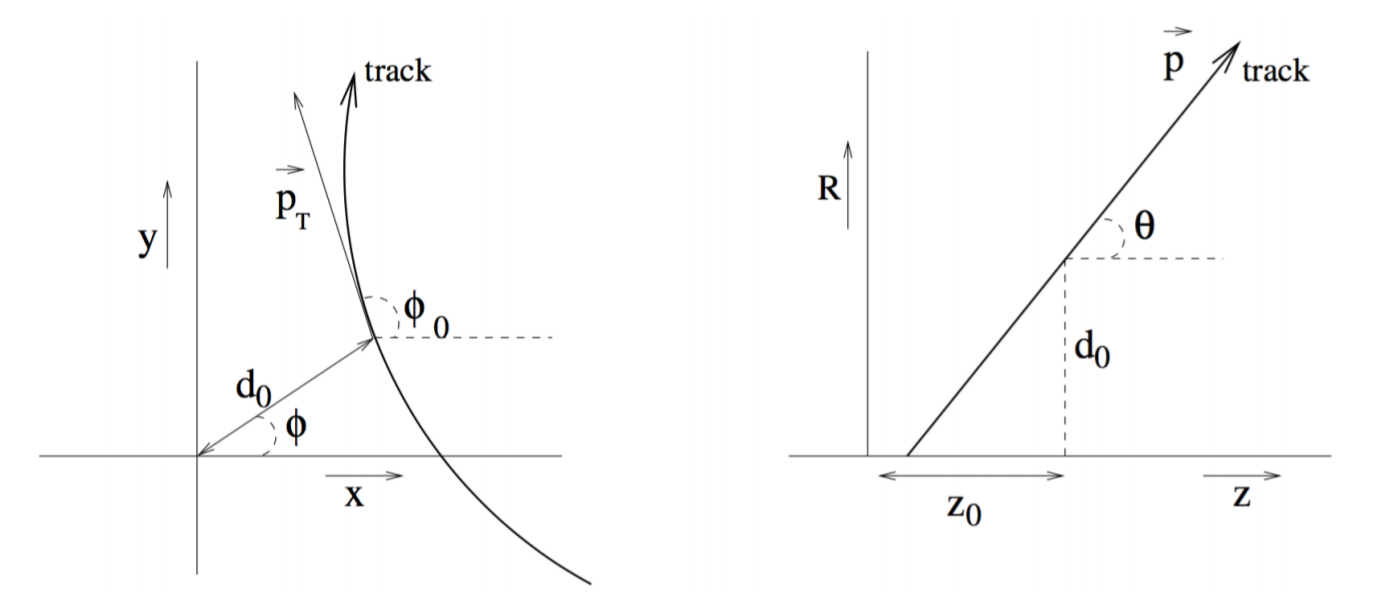
\includegraphics[width=0.9\textwidth]{figures/Simulation/track_parameter_2d.png}
  \caption{Schematic of the impact parameters of a track in the transverse plane (left)
and RZ-plane (right), as defined in the global ATLAS tracking frame\cite{Limper:1202457}.}
  \label{fig:ele_d0z0}
\end{figure}

\textbf{Electron identification}

The electron identifications (ID) are applied to determine the reconstructed electron candidates are more signal-like or background-like objects.
The ID algorithms make use of quantities of related variables from electron cluster and track measurements including calorimeter shower shapes, track properties, 
as well as variables measuring bremsstrahlung effects for distinguishing signal from background.
Taking the advantage of new IBL in run-2, the number of hits in this innermost pixel layer is utilized for discriminating between electrons and converted photons.
In addition, a likelihood method based on the TRT high-threshold hits is adopted to compensate the lower transition radiation absorption probability of the argon.

The baseline ID algorithm introduced for ATLAS run-2 data analysis if the likelihood-based (LH) method, which use a MVA technique to simultaneously evaluate several properties of electron candidates when making a decision.
The LH method utilizes the probability density functions (PDFs) of signal and background as the input discriminating variables.
Based on these PDFs, it can calculate an overall probability for the object to be signal or background.
Then the probabilities of signal and background are combined together into a discriminant $d_{\mathcal{L}}$:
\begin{equation}
	d_{\mathcal{L}} = \frac{\mathcal{L}_{S}}{\mathcal{L}_{S} + \mathcal{L}_{B}},
	~~ \mathcal{L}_{S(B)}(\vec{x}) = \prod_{i=1}^{n} P_{s(b),i}(x_{i})	
\end{equation}
where $\vec{x}$ denotes the vector of discriminating variables and $P_{s(b),i}(x_{i})$ represents the value of signal (background) PDF of the $i^{th}$ varaible as $x_{i}$.

Three levels of working points (WPs) for electron ID are provided: \textit{Loose}, \textit{Medium} and \textit{Tight}, in order of incresing background rejection.
Samples selected by a looser WP are subsets of a tighter one, eg. the electrons passing Medium can all be selected by Loose.
The ID efficiency varys as function of electron energy ($E_{T}$) as shown in figure~\ref{fig:ele_IDeff}.
For evaluations, the electron candidates from MC simulation of $Z \rightarrow ee$ decays (dijet) is used as signal (background).
Depending on the working point, the signal (background) efficiencies for reconstructed electron candidates at $E_{T} = 25 GeV$ are in the range from 78 to 90\% (0.3 to 0.8\%), and increase (decrease) with $E_{T}$.
\begin{figure}[!htb]
  \centering
  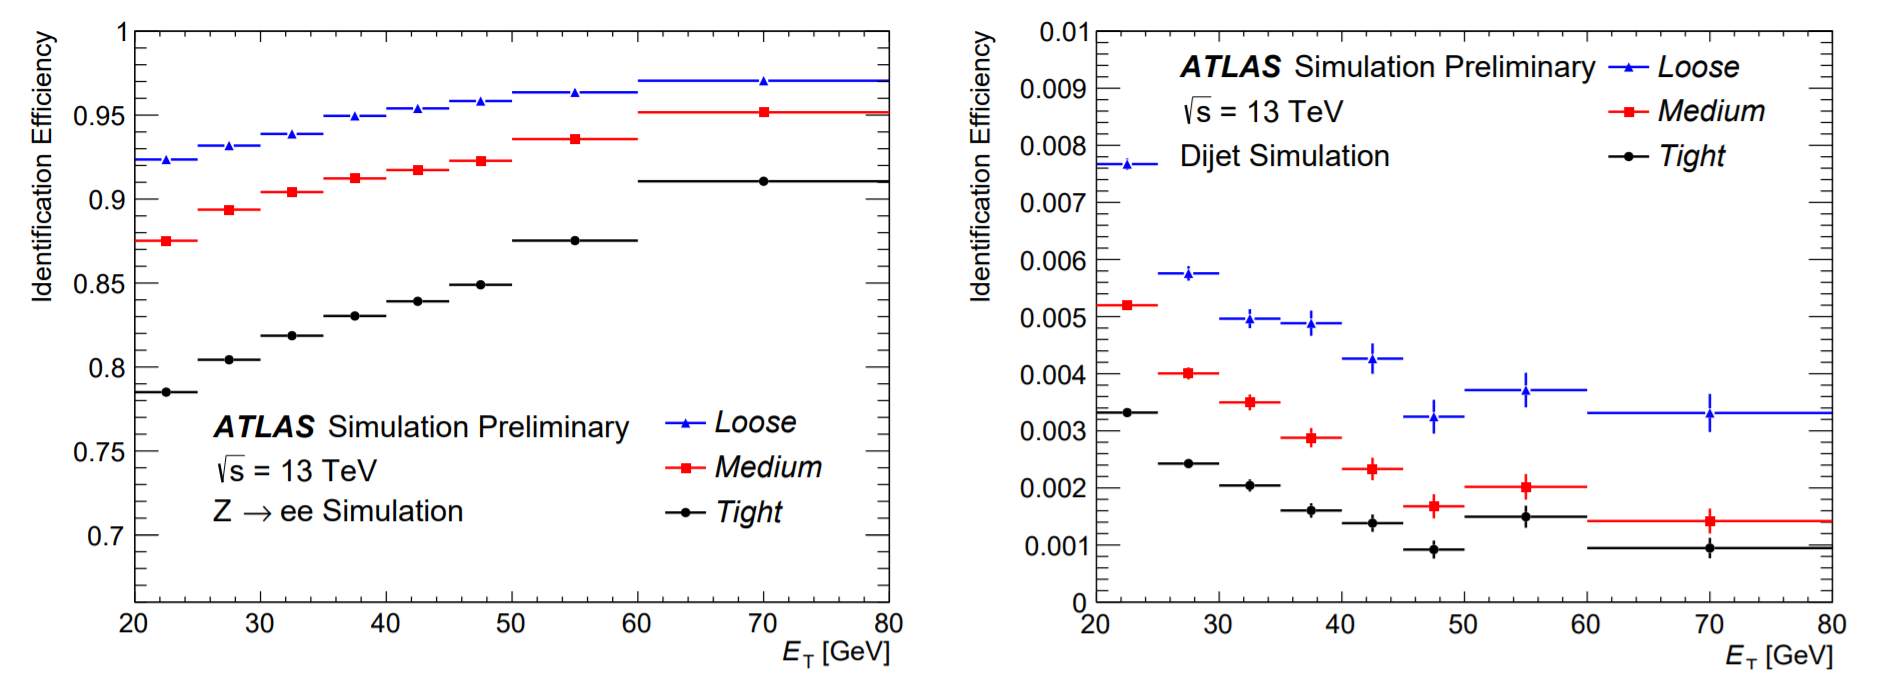
\includegraphics[width=0.9\textwidth]{figures/Simulation/ele_id_eff.png}
  \caption{The efficiencies of three electron ID WPs from $Z \rightarrow ee$ (left) events and hadrons misindentified as electrons estimated using dijet MC samples (right).}
  \label{fig:ele_IDeff}
\end{figure}

\textbf{Electron isolation}

In addition to the ID criteria, most analyses have electron isolation requirement to further distinguish signal from background.
To quantify the energy of particles around the electron candidate, the isolation variables can help to separate the prompt electron from other, non-isolated electron candidates, like the electrons from converted photons or from heavy flavour hadron decays.
There are two kinds of discriminating variables that have been designed:
\begin{itemize}
	\item \textbf{Calorimeter-based variable:} $E_{T}^{cone0.2}$. It's defined as the sum of transverse energies of topogical clusters\cite{Aad:2016upy}, calibrated at EM scale within a cone of $\Delta R = 0.2$ around the candidate electron cluster. It only consider the clusters with positive reconstructed energy. Besides, a correction as a function of $(E_{T}, \eta)$ values is then applied to account for the electron energy leakage outside the cluster.
	\item \textbf{Track-based variable:} $p_T{}^{varcone0.2}$. It's calculated as the sum of all transverse monmentum of all satisfied tracks within a cone of $\Delta R = min(0.2, 10 GeV/E_{T})$ around the candidate electron track. For the sum calculation, it requires the tracks are originating from the reconstruction PV of hard collision, and exclude the associated tracks of electron itself.
\end{itemize}
Based on the values of $E_{T}^{cone0.2}/E_{T}$ and $p_{T}^{varcone0.2}/E_{T}$, a serious of working points with different selection requirements are defined.
The resulting WPs are divided into two kinds:
\begin{itemize}
	\item Efficiency targeted working points: varying requirements to obtain a certain isolation efficiency, which can either be a constant or as a funtion of $E_{T}$.
	\item Fixed requirement working points: set the constant upper thresholds on isolation variables.
\end{itemize}
The distribution of two discriminating variables are shown in figure~\ref{fig:ele_iso} for $ZZ \rightarrow ee$ events with $E_{T} > 27 GeV$ and satisfying \textit{Tight} requirement.
\begin{figure}[!htb]
  \centering
  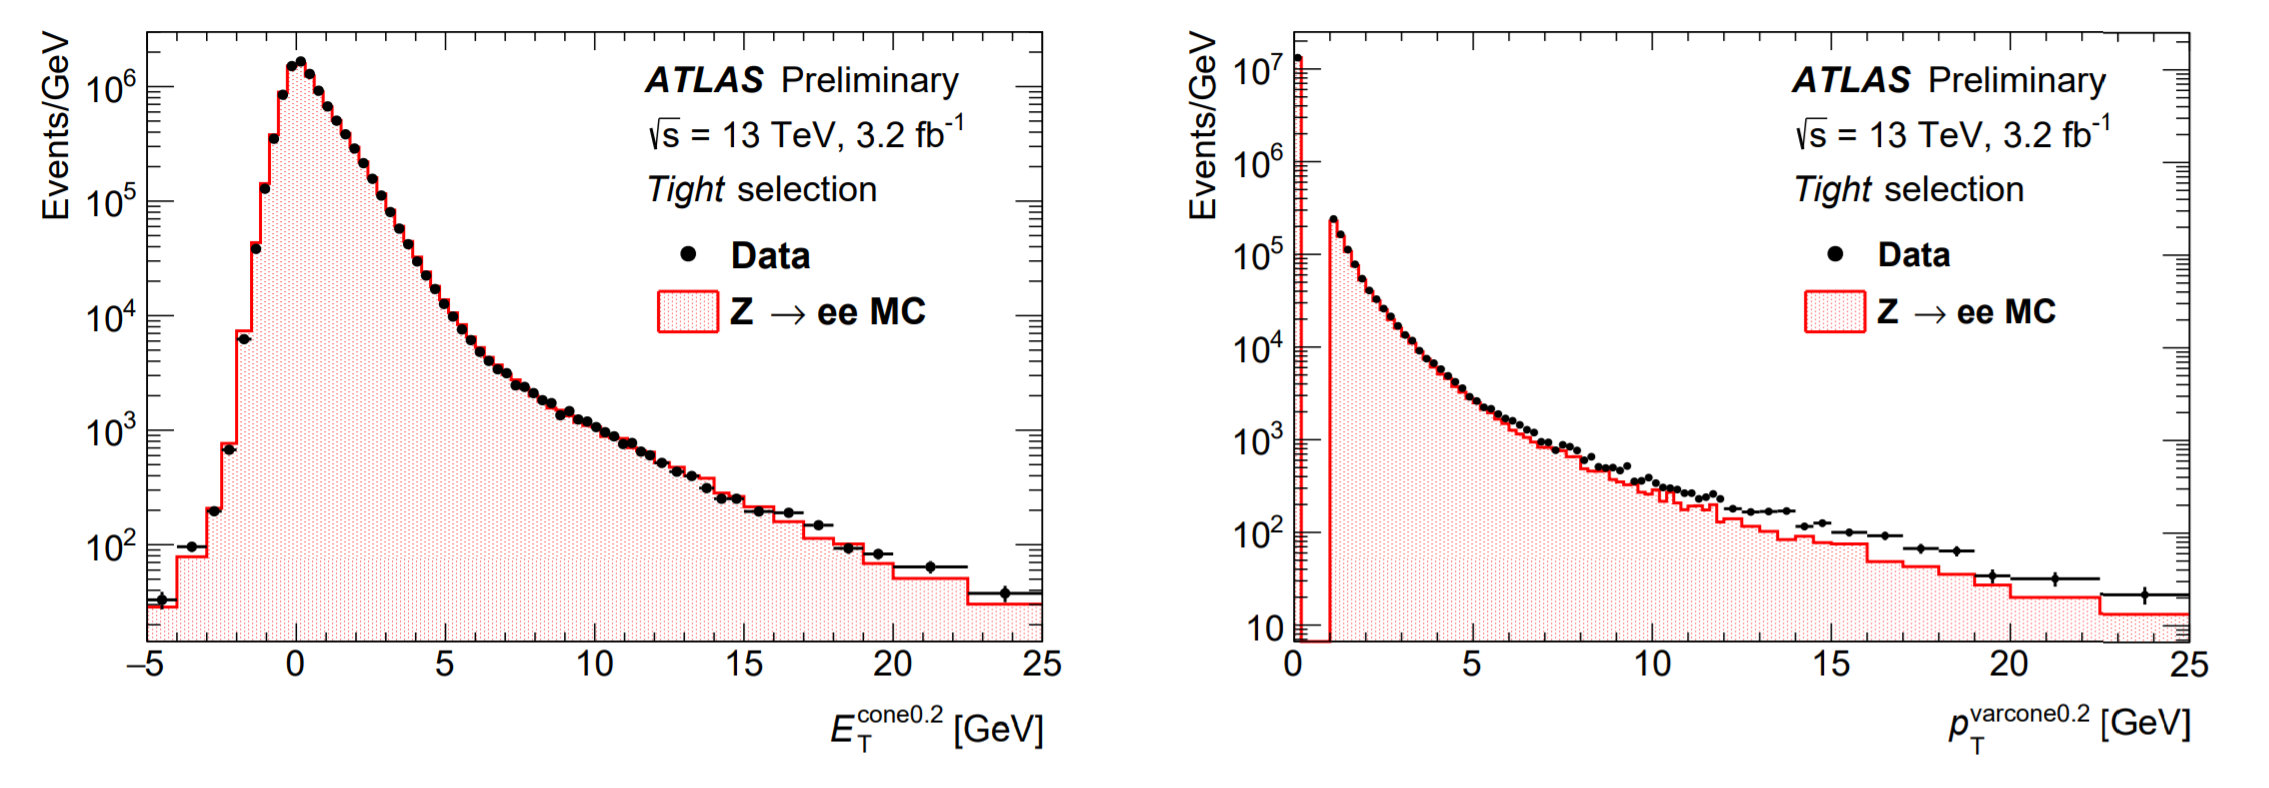
\includegraphics[width=0.9\textwidth]{figures/Simulation/ele_iso.png}
  \caption{Distributions of $E_{T}^{cone0.2}$ (left) and $p_{T}^{varcone0.2}$ (right) for electrons from $ZZ \rightarrow ee$ events in data and MC simulation. The simulated events (full histograms) are normalized to data.}
  \label{fig:ele_iso}
\end{figure}


\subsection{Muon}
\label{sec:muon}

Muons are distinctive signatures in final states of many physics analyses at the LHC which include the Higgs analyses, SM measurements and BSM searches and so on. 
High performance of muon reconstruction and identifications are crucial.
This section briefly describes some more details of the reconstruction, identification and isolation of muon.

\textbf{Muon reconstruction}

Muon reconstruction is firstly performed in inner detector (ID) and muon spectrometer (MS) independently as given in section~\ref{sec:track}.
The information from each individual detectors are then combined together to form the muon tracks for physics analyses.
The combined ID-MS reconstruction is developed according to several algorithm based on the information from ID, MS and calorimeters.
Four different muon types are defined\cite{Aad:2016jkr}:
\begin{itemize}
	\item \textbf{Combined (CB) muons:} a combined track is formed by using the reconstructed tracks performed independently in ID and MS with a global refit. To improve the fit quality, the hits from MS may be added to or removed from the track. The outside-in pattern recognition is utilized for the reconstruction of most muons, in which the muons are first reconstructed in MS and then extrapolated inward to match the ID track. In the meantime, the inside-out pattern is also used as a complementary method.
	\item \textbf{Segment-tagged (ST) muons:} a reconstructed track in ID is defined as muon, if it can associated with at least one track segment in MDT or CSC chambers. These ST muons are used when they can only pass across one layer of MS chambers due to their low $p_{T}$ or falling into regions with less MS acceptance.
	\item \textbf{Calorimeter-tagged (CT) muons:} a reconstructed track in ID is categorized as muon if it's matched to the energy deposit in calorimeter which is recognized with a minimum-ionizing particle. This CT muons have lowest purity amount all types of muons, but it covers the region where ATLAS muon spectrometer is only partially constructed. For the region of $|\eta| < 0.1$ and $15 GeV < p_{T} < 100 GeV$, the identification of CT muons are optimal.
	\item \textbf{Extrapolated (ME) muons:} the muon is reconstructed based only on the MS track and a loose requirement of originating from the interaction point. In general, this type of muon needs to pass at least two (three) layers of MS chambers to provide a track measurement in barrel (forward) region. ME muons are designed to extend the acceptance for muon reconstruction into the region $2.5 < |\eta| < 2.7$ where ID doesn't cover.
\end{itemize}

Before collecting those muons for physics analyses, overlap removals are performed between different muon types with the priority of CB > ST > CT, if two types of muons share the same ID track.
Besides, the overlaps with ME muons are resolved by analyzing the track hit content, and selecting the track with better fit quality and larger number of hits.

\textbf{Muon identification}

After reconstruction, the muon identification is then performed to further discriminate between signal and background, especially to suppress backgrounds from pion and kaon decays by requiring prompt muons with high efficiency and guaranteeing a robust momentum measurement.
The muon identification is defined by using the fit quality of combined track. 
The variables utilized in judgement for CB tracks include:
\begin{itemize}
	\item \textit{q/p significance}, the absolute difference between q/g (charge over momentum) of muons measured in ID and MS divided quadratic sum of their corresponding uncertainties;
	\item \textit{$\rho'$}, the absolute value of difference between the $p_{T}$ (transverse momentum) measured in ID and MS, divided by the $p_{T}$ of combined track;
	\item \textit{Nomalized $\chi^{2}$} of the combined track fit;
	\item \textit{Number of hits in ID and MS}
\end{itemize}
In addition, some new variables used for \textit{LowPt} muon working point what will be described below include\cite{Zheng:2649299}:
\begin{itemize}
	\item \textit{Momentum balance significance (MBS) } is computed as momentum difference between the ID and MS standalone measurements with respect to the uncertainty $\sigma$ on energy lost in the calorimeter system.
	\item \textit{Scattering neighbor significance (SNS)} is defined to estimated the significance of a change in trajectory along the track, expected in the presence of a hadron decaying to a muon.
	\item \textit{Scattering curvature significance (SCS)} is defined as the normalized integral of the scattering angle significances, corrected for large kinks along the trajectory.
\end{itemize}

Five selection levels are developed to satisfy the different needs for different physics goals: \textit{LowPt}, \textit{Loose}, \textit{Medium}, \textit{Tight} and \textit{HighPt}.
The \textit{Tight}, \textit{Medium}, \textit{Loose} are subsets from the tighter one to looser one.
More detailed definition of each working point is given as follow:
\begin{itemize}
	\item \textit{Loose:} this working point is designed to maximize the reconstruction efficiency while keeping good-quality of muon tracks. And they are specifically developed for reconstructing the Higgs boson candidates from four-lepton final states. All four muon types are used for this selection level. The CB and ME muons passing Medium WP that will mentioned below are all included into Loose category. In addition, the CT and ST muons are restricted to $|\eta| < 0.1$ region.
In the range of $|\eta| < 2.5$, around 97.5\% Loose muons are CB muons, and about 1.5\% are CT while remaining 1\% are ST muons.
	\item \textit{Medium:} this working point is the default criteria of muon identification in ATLAS. This selection minimizes the systematic uncertainties of muon reconstruction and calibration. In this category, we only use CB and ME muons. For CB muons, at least 3 hits in at least two layers of MDT is required, except $|\eta| < 0.1$ region, in which tracks with $\geq 1$ MDT layer but $\leq 1$ MDT hole layer are allowed. For ME muons, at least 3 MDT/CSC layers is required.
Furthermore, a loose cut on the compatibility between measured momentum in ID and MS is applied to reduce the fake muons from hadrons misidentification. Besides, the q/p-significance is required to be less than 7.
	\item \textit{Tight:} this working point is used to maximize the purity of muons but with sacrifice of some selection efficiency. Only CB muons with hits in $\geq 2$ stations of MS and passing Medium criteria are selected.
In addition, the normalized $\chi^{2}$ of combined track fit should be smaller than 8. Then, a two-dimensional cut of q/p-significance and $\rho'$ is adopted as a function of muon $p_{T}$ to ensure tighter background rejection for momentum below 20 GeV, in which the fake rate is usually higher.
	\item \textit{High-$p_{T}$:} this set of selections aims to maximize the momentum resolution for tracks with $p_{T} > 100 GeV$ region. The selection is especially optimized for searching high-mass Z' and W' resonances. CB muons satisfying Medium selection and with $\geq 3$ hits in 3 MS stations are chosen. The specific region in MS where alignment is suboptimal are removed as a precaution.
	\item \textit{Low-$p_{T}$:} this type of muon is newly designed for physics analyses with ATLAS software release version 21. It's designed to obtain a optimal muon identification with very low transverse momentum of $3 GeV < p_{T} < 5 GeV$, which is crucial for B-physics measurement in ATLAS. 
	In this muon requirement, only CB muons are used. In the range of $|\eta| < 1.3$, it requests muons hit at least one MS station; in $1.3 < |\eta| < 1.55$, a least two MS stations are required; while in region of $|\eta| > 1.55$, \textit{Medium WP} is required. In addition, cuts are applied to suppress fakes: |MBS| < 3.0, |SNS| < 3.0 and |SCS| < 3.0.
\end{itemize}

Figure~\ref{fig:muon_id_eff} and \ref{fig:muon_id_lowpt} show the selection efficiency of different muon identification working points. For \textit{Medium}, \textit{Tight} and \textit{High-$p_{T}$:}, $Z \rightarrow \mu\mu$ events with $p_{T} > 10 GeV$ are used for measurement. 
In addition, the top plot also shows the efficiency of the \textit{Loose} selection (squares), in which the Loose and Medium selections differ significantly in region of $|\eta| < 0.1$.
For \textit{LowPt}, $J/\Psi \rightarrow \mu\mu$ events with $3 GeV < p_{T} < 10 GeV$ are used for measurement.
\begin{figure}[!htb]
  \centering
  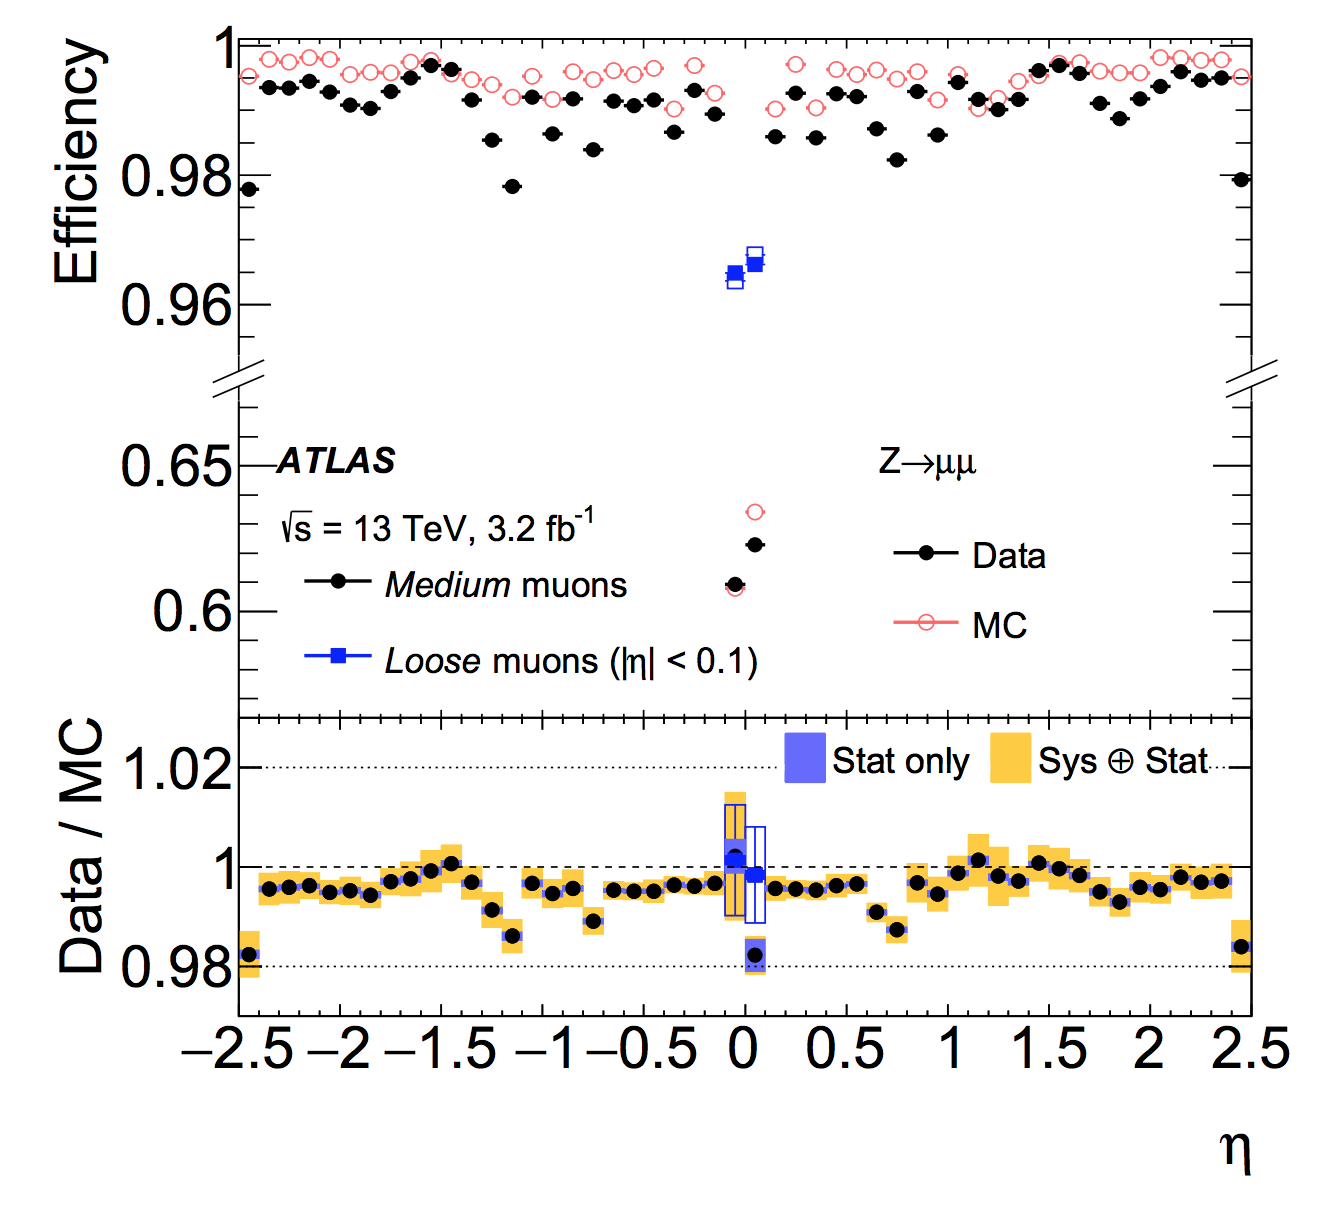
\includegraphics[width=0.42\textwidth]{figures/Simulation/muon_id_med.png} \\
  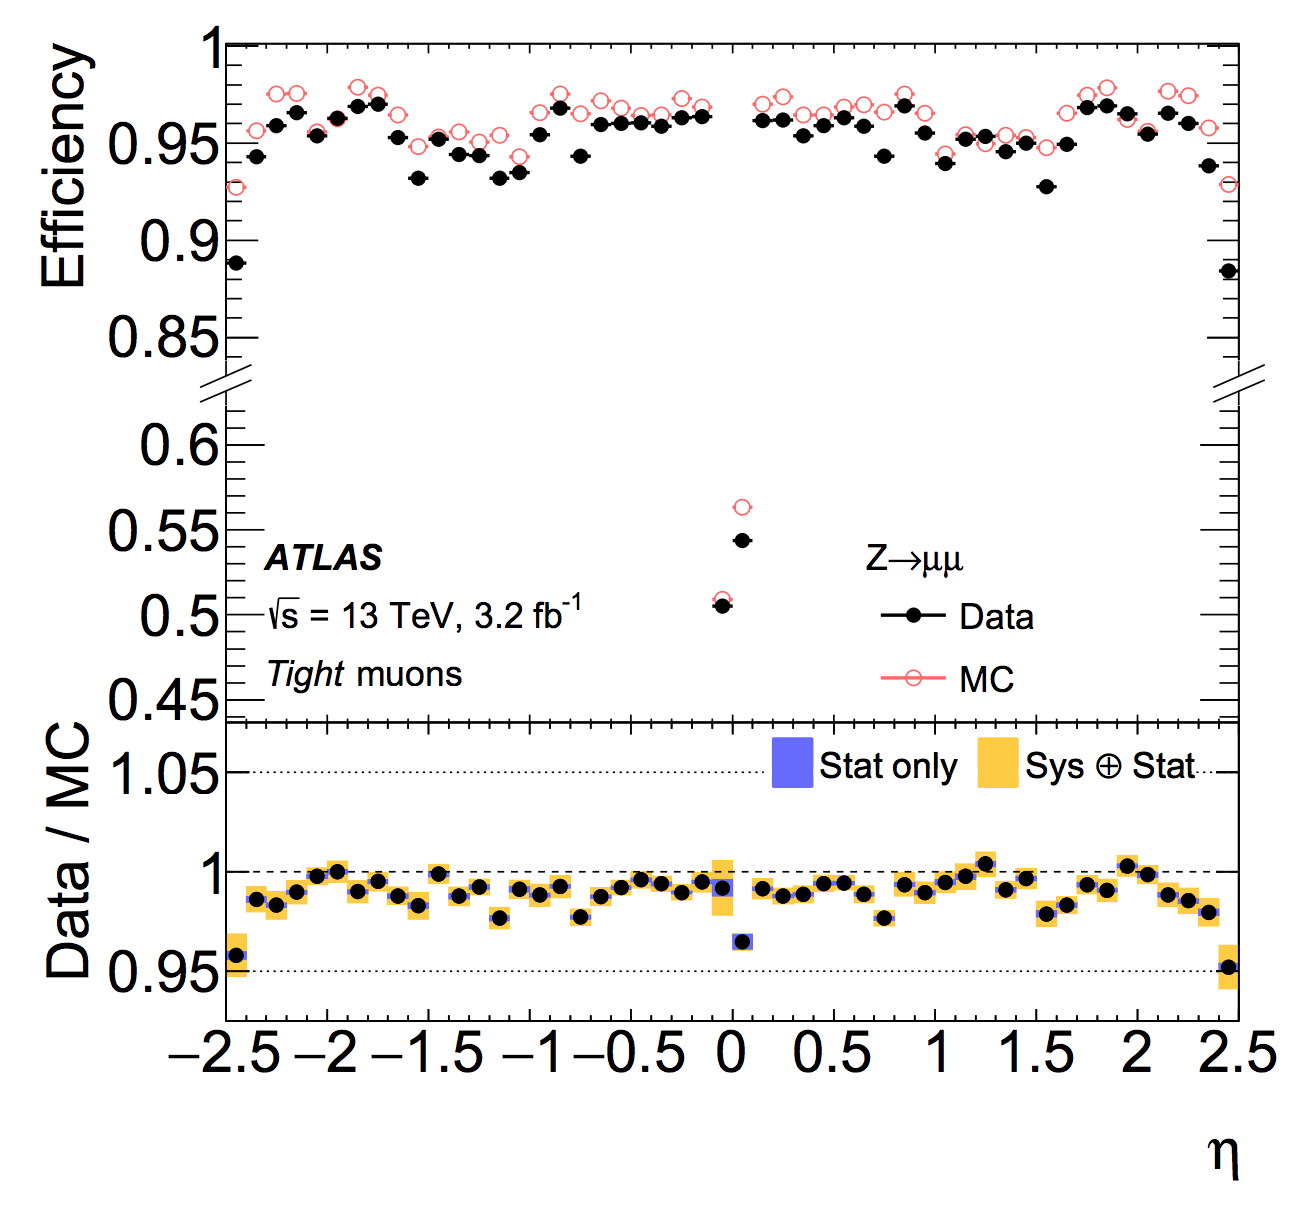
\includegraphics[width=0.42\textwidth]{figures/Simulation/muon_id_tight.png}
  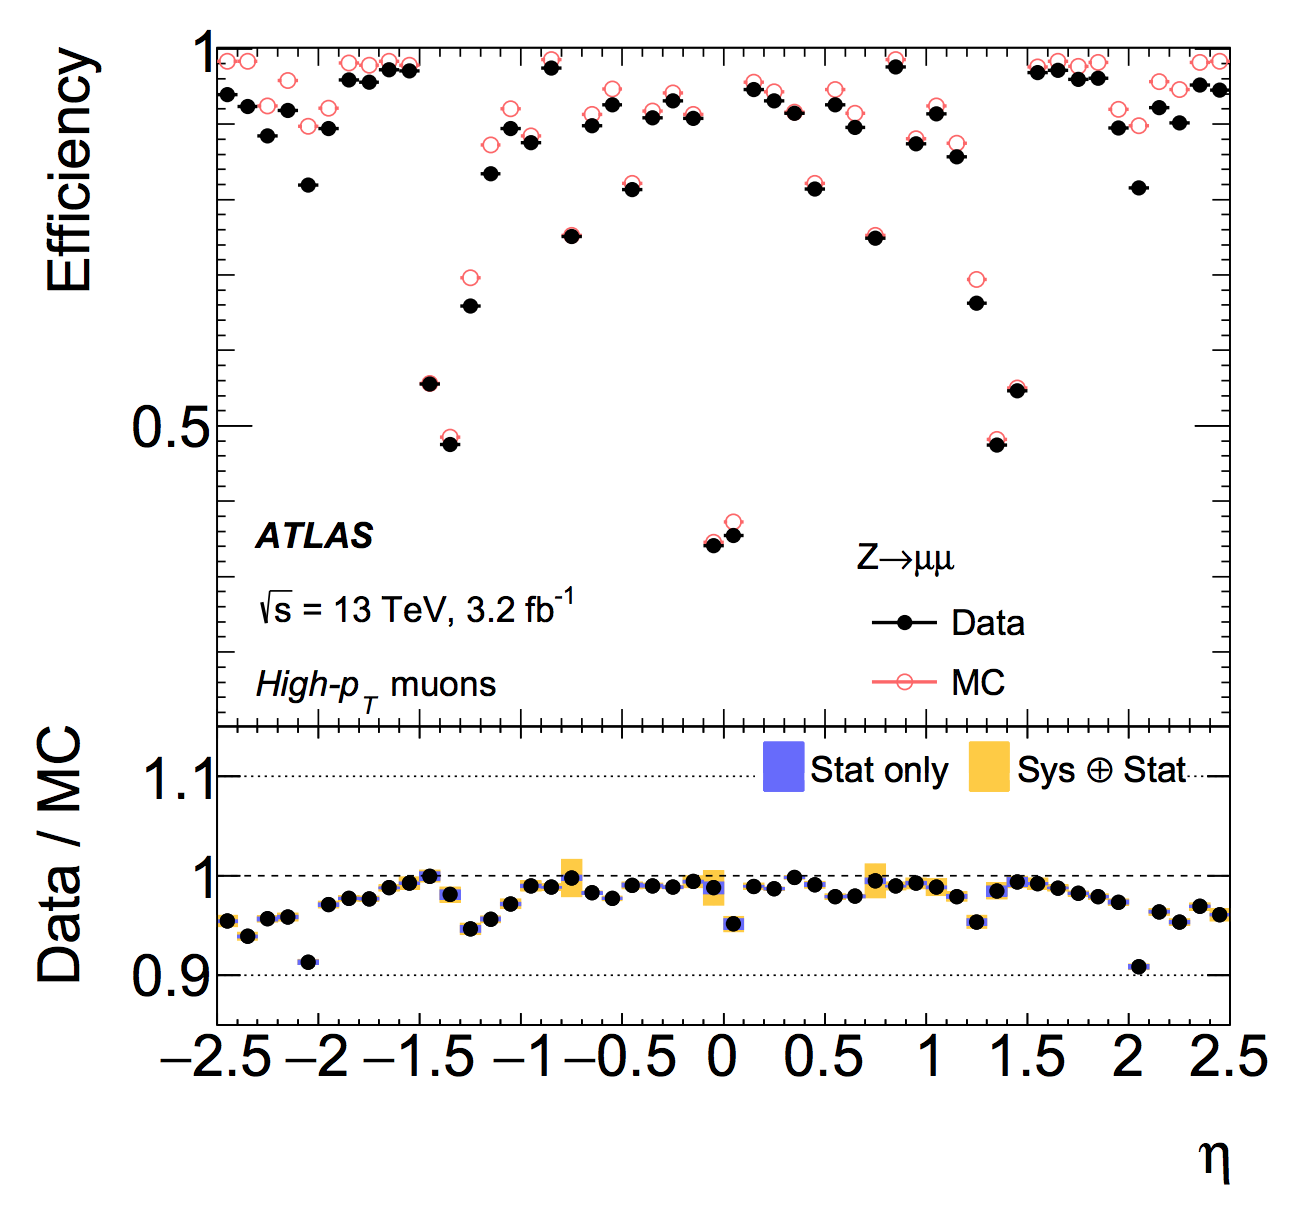
\includegraphics[width=0.42\textwidth]{figures/Simulation/muon_id_highpT.png}
  \caption{Muon reconstruction efficiency as a function of $\eta$ for: Medium (and Loose), Tight and High-$p_{T}$ working points.}
  \label{fig:muon_id_eff}
\end{figure}

\begin{figure}[!htb]
  \centering
  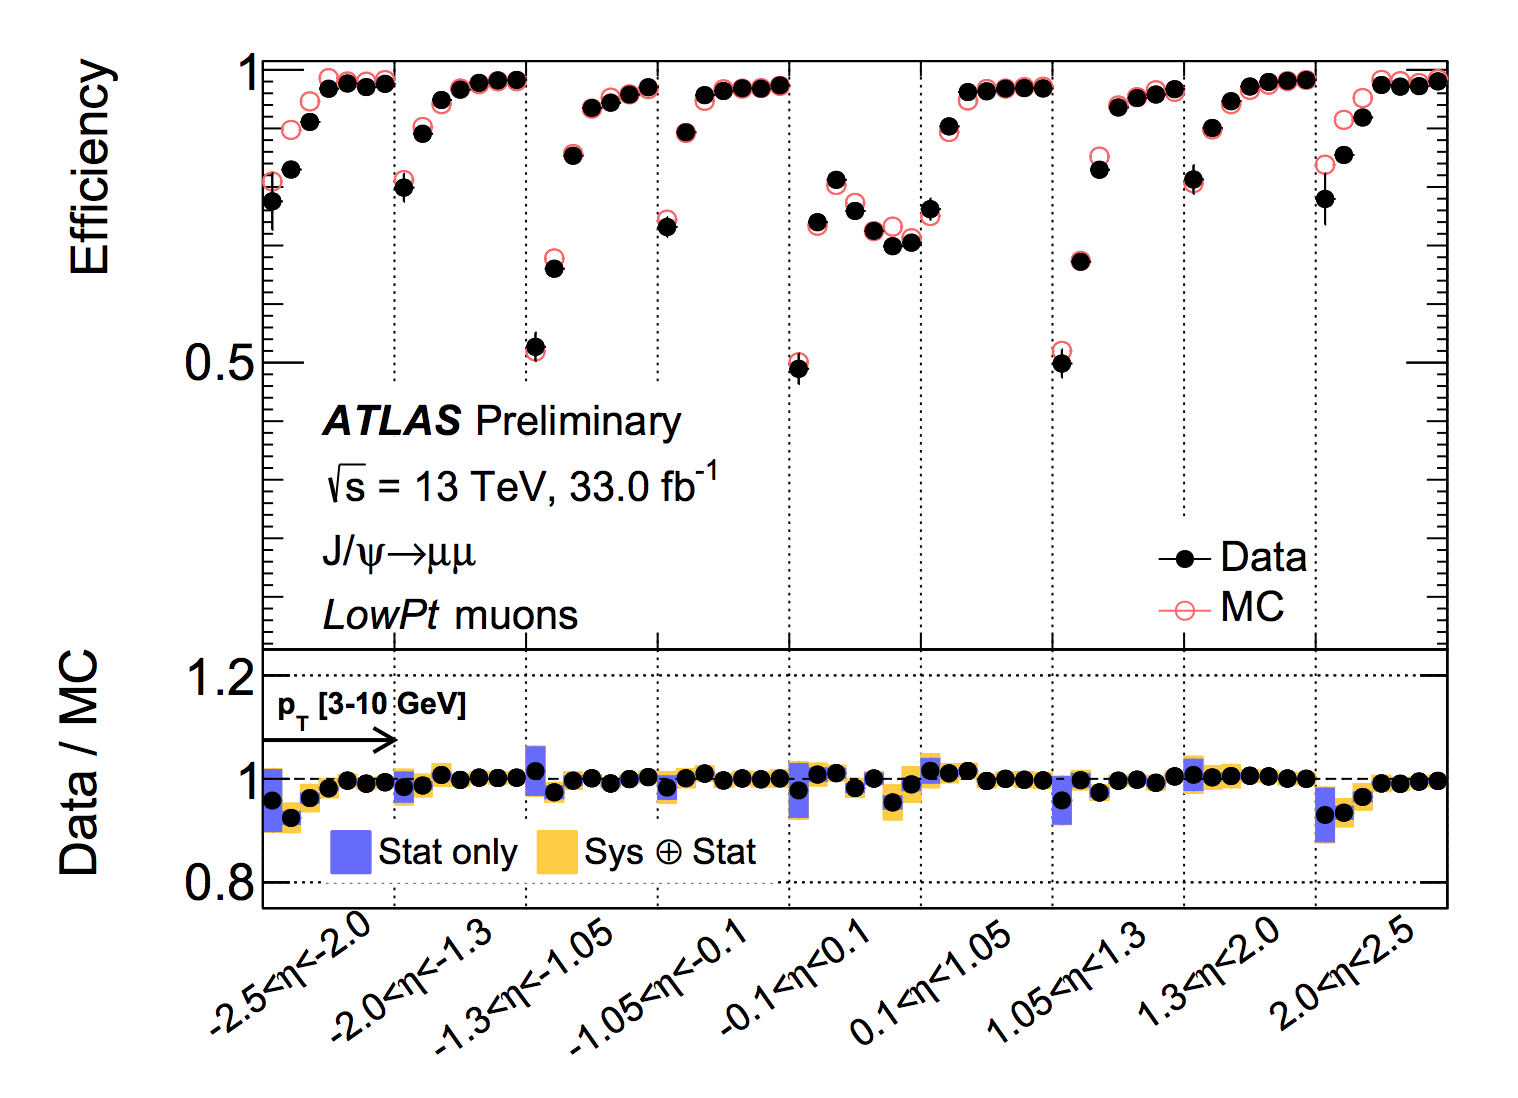
\includegraphics[width=0.5\textwidth]{figures/Simulation/muon_id_lowpT.png}
  \caption{Muon reconstruction efficiency for Low-$p_{T}$ working point as a function of $\eta$.}
  \label{fig:muon_id_lowpt}
\end{figure}

\textbf{Muon isolation}

Similar as electron, the muon isolation is used to further distinguish the prompt muon from non-prompt backgrounds.
There are also two types of isolation variables for muon:
\begin{itemize}
	\item \textbf{Calorimeter-based variable:} $E_{T}^{topocone20}$. It's defined as the sum of the transverse energy of topological clusters within a cone of size $\Delta R = 0.2$ around the candidate muon, after subtracting the contribution from the energy deposit of the muon itself and correcting for pile-up effects. The contributions from pile-up and underlying events are computed using the ambient energy-density technique\cite{CACCIARI2008119} and are corrected on an event-by-event basis.
	\item \textbf{Tracked-based variable:} $p_{T}^{varcone30}$. It's computed as the scalar sum of the transverse momenta of the tracks with $p_{T} > 1 GeV$ in a cone size of $\Delta R = min(10 GeV/p_{T}^{\mu}, 0.3)$ around the candidate muon whose transverse momenta is $p_{T}^{\mu}$ after excluding the muon track itself. This $p_{T}$-dependent cone size can help to improve the performance for muons produced in the decay of particles with a large transverse momentum.
\end{itemize}

Then the isolation selections are applied based on \textit{relative isolation variables}, 
which are computed as the ratio of the track- or calorimeter-based isolation variables to the transverse momentum of the muon.
Figure~\ref{fig:muon_iso} shows the distribution of those relative isolation variables by using $Z \rightarrow \mu\mu$ events and passing \textit{Medium} identification criteria.
\begin{figure}[!htb]
  \centering
  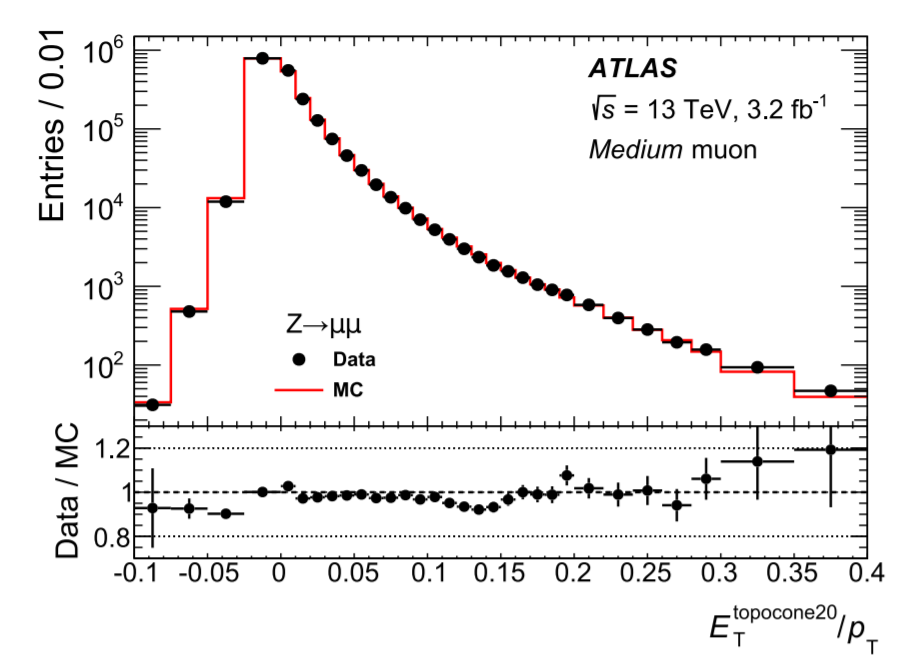
\includegraphics[width=0.42\textwidth]{figures/Simulation/muon_iso_calo.png}
  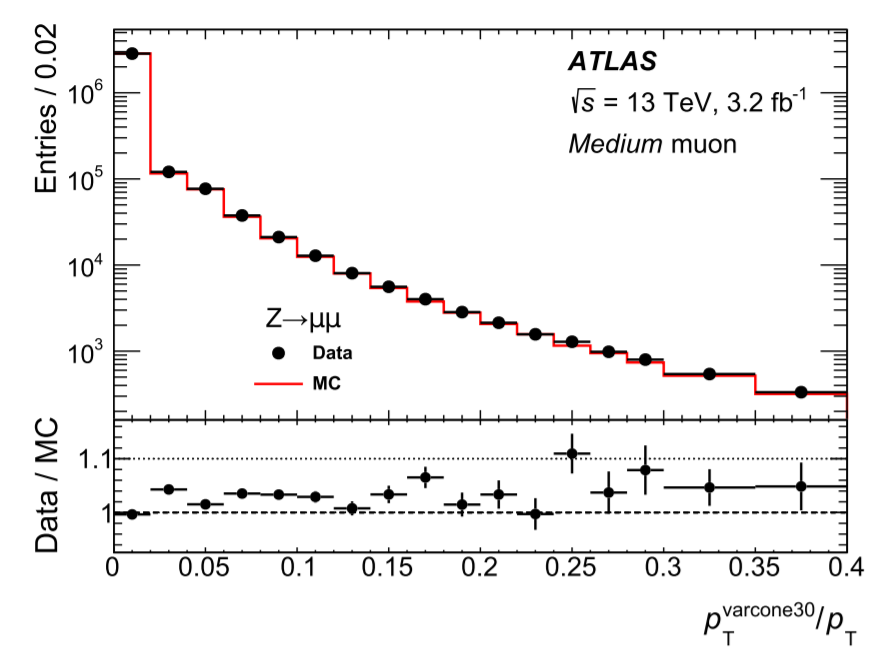
\includegraphics[width=0.42\textwidth]{figures/Simulation/muon_iso_track.png}
  \caption{Distributions of the calorimeter-based (right) and the track-based (left) relative isolation variables measured in $Z \rightarrow \mu\mu$ events. }
  \label{fig:muon_iso}
\end{figure}

\subsection{Jets}
\label{sec:jet}

Jets are another important features for many physics analyses at the LHC, and especially the key signatures for vector boson fusion/scattering (VBF/VBS) processes.
In ATLAS detector, jets are reconstructed as groups of topologically associated energy deposits in the calorimeters, 
tracks associated with charged particles measured in the inner tacking detector, or simulated particles.
This section will introduce the jet reconstruction, jet energy scale (JES) calibration and the b-jet tagging technical.

\textbf{Jet reconstruction}

Jets are reconstructed using anti-$k_{t}$ algorithm\cite{Cacciari_2008} and with radius parameter of $R = 0.4$ in most cases.
The \textsc{FastJet} software package\cite{Cacciari2012} is utilized for jet finding and reconstruction.
A collection of four-vectors are used as inputs at each combination step in jet clustering, 
the total four-momentum is therefore computed as the sum of four-vector of all its constituents.
There are three types of jets in ATLAS:
\begin{itemize}
	\item \textit{Truth jets:} the inputs to jet algorithm are simulated particles.
	\item \textit{Track jets:} the inputs are charged tracks measured from inner detector.
	\item \textit{Calorimeter jets:} the inputs are energy deposits in calorimeters.
\end{itemize}
Figure~\ref{fig:jet_reco_overview} shows the schematic of ATLAS jet reconstruction.
\begin{figure}[!htb]
  \centering
  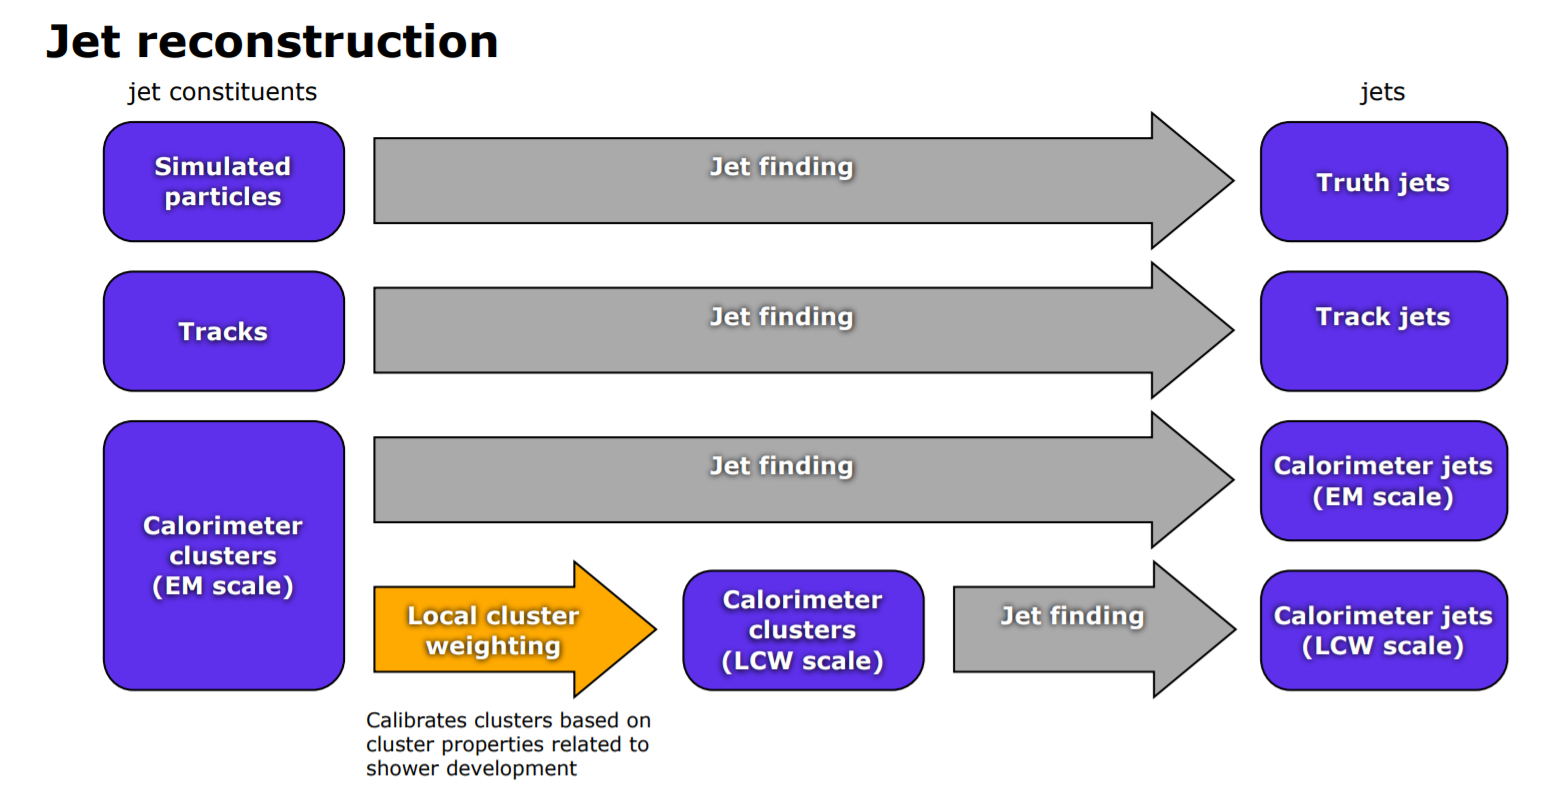
\includegraphics[width=1.0\textwidth]{figures/Simulation/threetypes_jet_reco.png}
  \caption{A overview schematic of ATLAS jet reconstruction\cite{Aad:2014bia}.}
  \label{fig:jet_reco_overview}
\end{figure}

The \textit{calorimeter jets} are reconstructed using a set of three-dimensional, positive-energy topological clusters (topo-clusters) made of calorimeter cell energies as input to the anti-$k_{t}$ algorithm\cite{Aaboud:2017jcu}.
Topo-clusters are built from near-by calorimeter cells that contains a significant energy above a noise threshold,
which is estimated from measurements of calorimeter electronic noise and simulated pile-up noise.
Those calorimeter cell energies are measured at electromagnetic energy scale (EM scale) corresponding to the energy deposited by electromagnetically interacting particles. 
And jets passing a \pt threshold of 7 GeV are reconstructed with the anti-$k_{t}$ algorithm.

The \textit{truth jets} are reconstructed also using anti-$k_{t}$ algorithm with $R = 0.4$ by using final-state, stable particles from MC simulation as inputs.
It requires the candidate particles with lifetime $c_{\tau} > 10mm$ and muons, neutrinos, and excludes particles from pile-up.
Truth jets with $p_{T} > 7 GeV$ and $|\eta| < 4.5$ are then used for jets calibration that will be mentioned later.

The \textit{track jets} are reconstructed from charged particles within the full acceptance of inner detector ($|\eta| < 2.5$).
The track reconstruction has been introduced in section~\ref{sec:track}.
Reconstructed jets with $p_{T} > 500 MeV$ and associated with primary vertex are then selected.
Tracks are assigned to jets using ghost association\cite{CACCIARI2008119}, a procedure that treats selected tracks as four-vectors of infinitesimal magnitude during the jet reconstruction and assigns them to the jet with which they are clustered.
In addition, muon track segments are used as a compensation for those uncaptured jet energy from energetic particles passing through the calorimeters without fully being absorbed.
The segments are tracks reconstructed from hits in MS and assigned to jets using the method of ghost association mentioned above as well.

\textbf{Jet energy scale calibration}

Figure~\ref{fig:jet_cali} depicts an overview of ATLAS jet calibration scheme for EM-scale calorimeter jets.
This procedure restores the jet energy scale to that of truth jets, which is reconstructed at the particle-level.
Each step of the calibration corrects the full four-momentum unless otherwise stated, scaling the jet \pt, energy, and mass.
\begin{figure}[!htb]
  \centering
  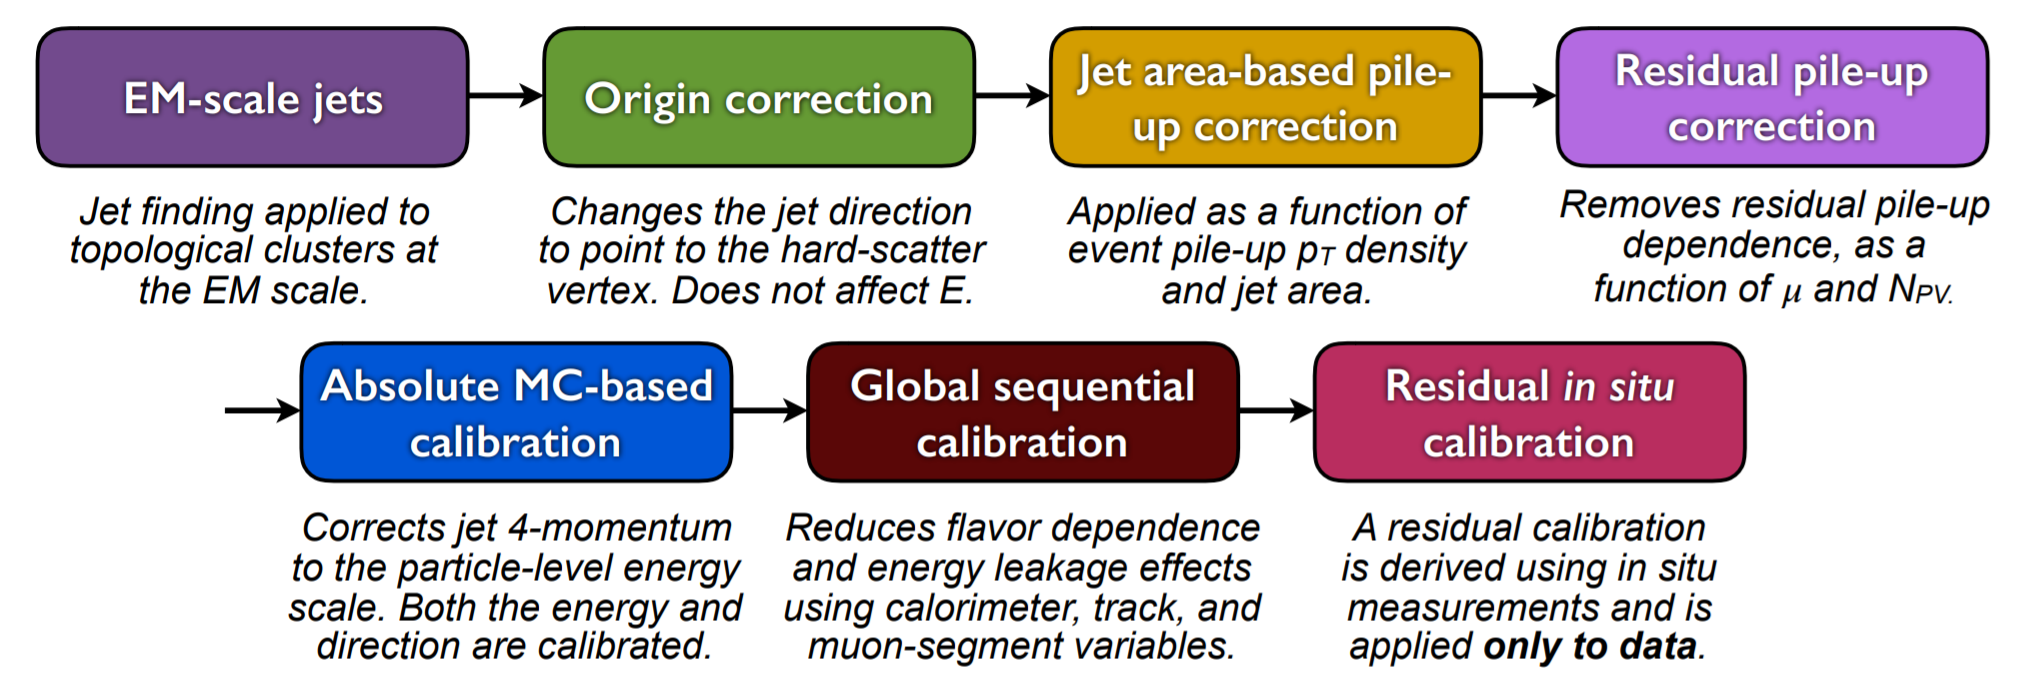
\includegraphics[width=1.0\textwidth]{figures/Simulation/jet_calibration.png}
  \caption{A overview schematic of ATLAS jet calibration\cite{Aaboud:2017jcu}.}
  \label{fig:jet_cali}
\end{figure}

First of all, the origin correction recompute the four-momentum of jets to point them to the hard-scatter primary vertex instead of the centre of detector, and in the meantime keep the jet energy unchanged.
This correction improves the $\eta$ resolution of jets for roughly 25\% at a jet $p_{T}$ of 20~\gev and > 5 times improvement for jet with $p_{T}$ above 200~\gev, 
as measured from the difference between reconstructed jets and truth jets in MC simulation.
Secondly, the pile-up correction is adopted to remove the excess energy due to in-time and out-of-time pile-up,
which consists of two processes: an area-based $p_{T}$ density subtraction applied on the top of each event; and a residual correction derived from the simulation.
Thirdly, the absolute JES calibration corrects the jet four-momentum to the particle-level energy scale, using truth jets in di-jet MC events.
Furthermore, the step of global sequential calibration use calorimeter, track and MS-based variables to reduce the flavor dependence and energy leakage effects.
Finally, the residual in situ calibration is adopted to correct jets in data by using well-measured objects eg. photons, Z bosons and calibrated jets.

\textbf{B-jet tagging}

Tagging of b-jets plays a important role in many physics analyses involving b- or t- quark.
On the other hand, lots of analyses need to apply b-jet veto to suppress top-antitop process.
There are three major types of algorithms that have been developed to distinguish b-jet from light-quark (u,d,s) jets~\cite{ATL-PHYS-PUB-2016-012}:
\begin{itemize}
	\item \textbf{Impact parameter based algorithms (IP2D and IP3D):} b-hadrons usually have long lifetime ($\sim$1.5 ps, $c_{\tau}\sim450~\mu$m), which leads to large impact parameter for tracks produced from b-hadron decay. The impact parameter taggers are developed based on these variables. The IP2D tagger makes use of the transverse impact parameter significance $d_{0}/\sigma(d_{0})$ as discriminant, while IP3D tagger uses two-dimensional discriminant of both transverse and longitudinal impact parameter significances: $d_{0}/\sigma(d_{0})$ and $z_{0}sin\theta/\sigma(z_{0})$.
	\item \textbf{Secondary vertex finding algorithm (SV1)} makes use of the secondary vertex formed by decay products of b-hadron within the jet. All track pairs within a jet are tested for a two-track vertex hypothesis, and removed if they are likely to originate from a long-live particle decay (eg. $K_{s}$ or $\Lambda$), hadronic interactions or photon conversions. After that, a new vertex is fitted with all tracks from remaining two-track vertices, and the outliers are removed from this set of tracks.
	\item \textbf{Decay chain multi-vertex algorithm (JetFitter)}\cite{Piacquadio_2008} exploits the topological structure of weak b- and c- hadron decays inside the jet and tries to reconstruct the full b-hadron decay chain. A Kalman filter is adopted to find a common line between primary vertex and b-/c- vertices, as well as their position in this line, which gives a approximated flight path for the b-hadron. In this approach, the b- and c-hadron vertices, whenever resolution allows, can be resolved, even when there is only a single track associated to them.
\end{itemize}
The final discrimination commonly used in many physics analyses is called \textbf{Multivariate Algorithm (MV2)}, which is based on Boosted Decision Tree (BDT) implemented in the TMVA package\cite{Speckmayer_2010} by combining the outputs from underlaying taggers mentioned above.
The MV2 was trained using jets in $t\bar{t}$ sample, where b-jets are treated as signal and c- and light-flavor jets are treated as backgrounds.
There are three kinds of MV2 depending on the fraction of c-jets in background for training: \textit{MV2c00}, \textit{MV2c10} and \textit{MV2c20}.
Figure~\ref{fig:jet_mv2} presents the output score of MV2c10 for different flavor jets.
\begin{figure}[!htb]
  \centering
  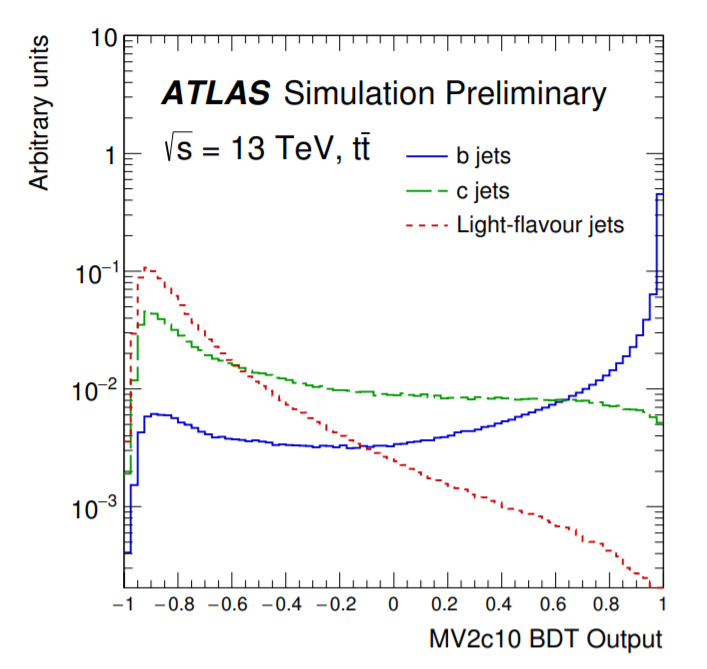
\includegraphics[width=0.5\textwidth]{figures/Simulation/jet_mv2c10.png}
  \caption{MV2c10 BDT output for b- (solid blue), c- (dashed green) and light-flavour (dotted red) jets in $t\bar{t}$ events\cite{ATL-PHYS-PUB-2016-012}.}
  \label{fig:jet_mv2}
\end{figure}

\subsection{Missing transverse energy}

Many interesting physics processes are with the inveloment of neutrinos.
Since they do not interact with any materials in the detector, neutrinos cannot be detected directly;
but instead, they can result in imbalance in the plane transverse to the beam axis, in which momentum conservation is assumed.
It is known as the missing transverse momentum denoted as $E_{T}^{miss}$,
which is obtained from the negative vector sum of the momenta of all particles detected in a proton-proton collision event.

The $E_{T}^{miss}$ is measured using selected, reconstructed and calibrated hard objects in an event.
Its x- and y- conponents can be calculated as follow\cite{Aaboud2018}:
\begin{equation} \label{eq:met_xy}
	E_{x(y)}^{miss} = E_{x(y)}^{miss, e} + E_{x(y)}^{miss, \gamma} + E_{x(y)}^{miss, \tau} + E_{x(y)}^{miss, jets} + E_{x(y)}^{miss, \mu} + E_{x(y)}^{miss, soft}
\end{equation}
where each object term is given by the negative vectorial sum of the momenta of the respective calibrated objects.
The calorimeter signals are associated with the reconstructed objects in the following order: electrons, photons, hadronically decaying taus, jets, muons.
The soft term is reconstructed from detected objects not match any hard object passing the selections, but associated with the primary vertex.
Details of applied selections for each term are summarized in table~\ref{tab:met_sele}.
\begin{table}[!htbp]
  \begin{center}
  \small
  \caption{Overview of the contributions to $E_{T}^{miss}$.}
  \label{tab:met_sele}
  \begin{tabular}{p{1cm}p{1.5cm}p{5cm}p{1.5cm}p{5cm}}
    \toprule
     \multicolumn{5}{c}{Objects contributing to $E_{T}^{miss}$} \\
     \hline
     Priority & Type & Selections & Variables & Comments \\
     \hline
     (1) & $e$          & $|\eta|<1.37~or~1.52<|\eta|<1.47 \newline p_{T}>10 GeV$ & $E_{T}^{miss, e}$      
         & all $e^{\pm}$ passing medium reconstruction quality and kinematic selections \\ 
     \hline
     (2) & $\gamma$     & $|\eta|<1.37~or~1.52<|\eta|<1.47 \newline p_{T}>25 GeV$ & $E_{T}^{miss, \gamma}$ 
         & all $\gamma$ passing tight quality and kinematic selections in reconstruction, and without signal overlap with (1) \\
     \hline
     (3) & $\tau_{had}$ & $|\eta|<1.37~or~1.52<|\eta|<1.47 \newline p_{T}>20 GeV$ & $E_{T}^{miss, \tau}$   
         & all $\tau_{had}$ passing medium reconstruction quality and kinematic selections, and without signal overlap with (1) and (2) \\
     \hline
     (4) & $\mu$        & $|\eta|<2.7 \newline p_{T}>10 GeV$ & $E_{T}^{miss, \mu}$
         & all $\mu$ passing medium quality and kinematic selections in reconstruction \\
     \hline
     (5) & jet          & $|\eta|<4.5 \newline p_{T}>60 GeV \newline 
			--- or --- \newline 
			2.4<|\eta|<4.5 \newline 20 GeV<p_{T}<60 GeV \newline
			--- or --- \newline
			|\eta|<2.4 \newline 20 GeV<p_{T}<60 GeV \newline JVT>0.59$ & $E_{T}^{miss, jet}$
         & all jets passing reconstruction quality (jet cleaning) and kinematic selections, and without signal overlap with (1)–(4) \\
     \hline
     (6) & ID track     & $p_{T}>400 MeV \newline 
			|d_{0}|<1.5 mm \newline 
			|z_{0}sin\theta|<1.5 mm \newline 
			\Delta R(track, e/\gamma cluster)>0.05 \newline 
			\Delta R(track, \tau_{had})> 0.2$       &  $E_{T}^{miss, soft}$ 
         & all ID tracks from the hard-scatter vertex passing reconstruction quality and kinematic selections, and not associated with any particle from (1), (3) or (4), or ghostassociated with a jet from (5) \\
    \bottomrule
  \end{tabular}
  \end{center}
\end{table}

Based on $E_{x(y)}^{miss}$, the magnitude of $E_{T}^{miss}$ and the azimuthal angle $\phi^{miss}$ are computed:
\begin{equation}
\begin{split}
	E_{T}^{miss} &= \sqrt{ \left(E_{x}^{miss}\right)^{2} + \left(E_{y}^{miss}\right)^{2} } \\
	\phi^{miss} &= arctan \left(E_{y}^{miss}/E_{x}^{miss}\right)
\end{split}
\end{equation}

In equation~\ref{eq:met_xy}, each objects are required to pass certain reconstruction and calibrated criteria and selections mentioned above before taken as inputs.

In figure~\ref{fig:met_dis}, left plot shows the $E_{T}^{miss}$ distribution for data and MC of $Z \rightarrow \mu\mu$ events, in which there is no genuine missing transverse momentum;
and right plot shows the $E_{T}^{miss}$ distribution for $W \rightarrow e\nu$ events that has genuine (true) missing transverse momentum due to real neutrino.
\begin{figure}[!htb]
  \centering
  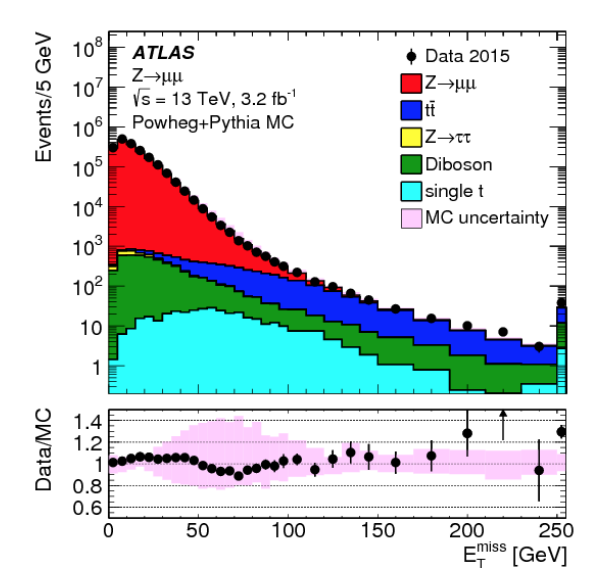
\includegraphics[width=0.42\textwidth]{figures/Simulation/met_Zmm.png}
  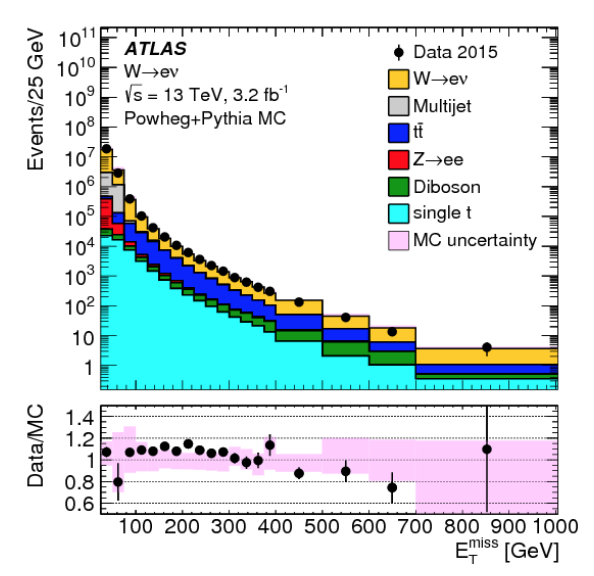
\includegraphics[width=0.42\textwidth]{figures/Simulation/met_Wev.png}
  \caption{Measured $E_{T}^{miss}$ distribution for $Z \rightarrow \mu\mu$ events (left) and $W \rightarrow e\nu$ events (right). }
  \label{fig:met_dis}
\end{figure}

